\documentclass[letterpaper,12pt]{article}

% Preamble
\usepackage[utf8]{inputenc}
\usepackage{amsmath, amssymb}
\usepackage{graphicx}
\usepackage{float}
\usepackage{hyperref}
\usepackage{subcaption}
\usepackage{xcolor, soul}
\usepackage{bm}
\usepackage{svg}
\usepackage{booktabs}

\usepackage[style=chem-acs]{biblatex}
\addbibresource{references.bib}
\usepackage{geometry}
\geometry{letterpaper, margin=1in}

\usepackage{tikz}

\usepackage{setspace}

\usepackage{titlesec}
\titleformat{\subsubsection}{\normalfont\normalsize}{\thesubsubsection}{1em}{}

\usepackage{caption}
\renewcommand{\figurename}{\textbf{\uppercase{Figure}}}
\renewcommand{\thefigure}{\arabic{figure}}
\captionsetup[figure]{
  labelsep=colon,
  labelfont={bf,small}, % Make label bold in caption
  textfont={small}, % Text in caption remains unbolded and small
  labelformat=default
  }
  \makeatletter
  \let\oldthefigure\thefigure
  \renewcommand{\thefigure}{\arabic{figure}}
  \makeatother
  
  
  \captionsetup[subfigure]{
    labelformat=parens,       % Add parentheses around the label
    labelsep=space,           % Add a space between the label and the caption
    textfont=normalfont,      % Use normal font for the caption text
    position=bottom,          % Position the label at the bottom of the subfigure
    format=plain              % Plain format for subfigure captions
    }
\renewcommand\thesubfigure{\Alph{subfigure}}


\usepackage{multicol}

\tikzstyle{block} = [rectangle, minimum width=2cm, minimum height=1cm,text centered, draw=black]
\tikzstyle{block_1} = [rectangle, minimum width=2cm, minimum height=1cm,text centered, draw=black, fill=blue!5]
\tikzstyle{block_2} = [rectangle, minimum width=2cm, minimum height=1cm,text centered, draw=black, fill=red!5]
\tikzstyle{arrow} = [thick,->,>=stealth]
\tikzstyle{arrow_2} = [very thick,->,>=stealth]
\tikzstyle{arrow_3} = [thick,->,>=stealth,dashed]
\tikzstyle{pfr} = [cylinder, draw, minimum height=4cm, minimum width=1cm, shape aspect=1, shape border rotate=180]
\usetikzlibrary{shapes.geometric}


% Title and author information
\title{Optimal control of axial dispersion tubular reactors with recycle: Addressing state-delay through transport PDEs}
\author{
  Behrad Moadeli \thanks{Department of Chemical and Materials Engineering, University of Alberta, Edmonton, Alberta, Canada, T6G 1H9} \thanks{Corresponding author. Email: moadeli@ualberta.ca} \and
  Guilherme Ozorio Cassol\footnotemark[1] \and
  Stevan Dubljevic \footnotemark[1] 
  }
  
\date{\today}

\begin{document}

\maketitle

\begin{figure}[htbp!]
  \centering
  \includegraphics*[width=\textwidth]{Figures/abstract_final.PNG}
  \caption*{\textbf{Graphical abstract:}
  The boundary-regulated distributed parameter system of an axial dispersion tubular reactor with delayed recycle is showcased, along with the optimal observer-based control strategy developed using a late-lumping method for its stabilization.}
\end{figure}

\newpage
\begin{abstract}
  The optimal control of an axial tubular reactor with a recycle stream is addressed as a key type of setting for distributed parameter systems in chemical engineering. The intrinsic time delay from the recycle process, thus far overlooked in relevant literature, is modelled as a transport partial differential equation (PDE), resulting in a system of coupled parabolic and hyperbolic PDEs. Utilizing the Danckwerts boundary conditions, the reactor is boundary-controlled with the control input at the inlet. A continuous-time optimal linear quadratic regulator is developed to stabilize the infinite-dimensional system, employing a late lumping approach in order to preserve the properties of the original infinite dimensional system in controller design. The full-state feedback regulator is designed by solving the operator Riccati equation (ORE), leveraging the system's Riesz-spectral properties. To address practical limitations of full-state feedback, a Luenberger observer is also proposed, enabling state reconstruction from boundary measurements.
  Numerical simulations are conducted to evaluate the proposed control strategies. The results demonstrate that the full-state feedback regulator effectively stabilizes the system. A comparison is made between two configurations where different numbers of eigenmodes were selected to design the controller. The observer-based regulator also stabilizes the system successfully using merely output measurements, effectively overcoming the challenge of limited state access. \\ \, \\
  \textit{Keywords: distributed parameter systems, tubular reactors, recycle, optimal control, state delay}
\end{abstract}

\newpage
% \tableofcontents
% \newpage
      
\onehalfspacing
% \begin{multicols}{2}

  \section{INTRODUCTION}

Many chemical, petrochemical, and biochemical unit operation processes are modelled as distributed parameter systems (DPS). When these processes are described using first-principle modeling, they result in a class of partial differential equations (PDEs) to effectively capture diffusion, transport, and reaction phenomena, leading to infinite-dimensional state space representations \autocite{ray1981advanced}. This characteristic presents significant challenges, making the control and estimation of DPS inherently more complex than finite-dimensional systems. Two primary methods have emerged for addressing DPS control. One is early lumping, which approximates the infinite-dimensional system with a finite-dimensional model \autocite{davison1976robust, francis1977linear}. While this method enables the use of standard regulator design techniques, mismatches between the dynamical properties of the original DPS and the approximate lumped parameter model can occur, negatively affecting the performance of the designed regulator \autocite{moghadam2012infinite}. The second method is late lumping, which directly tackles the infinite-dimensional system before applying numerical solutions. This approach introduces a challenging yet fertile direction of research, leading to many meaningful contributions that address various aspects of control and estimation of infinite-dimensional systems.

Among notable studies utilizing late lumping method for control of convection-reaction chemical systems resulting in first order hyperbolic PDEs, \Citeauthor{christofides1998robust} explored the robust control of quasi-linear first-order hyperbolic PDEs, providing explicit controller synthesis formulas for uncertainty decoupling and attenuation \autocite{christofides1998robust}. \Citeauthor{krstic2008backstepping} extended boundary feedback stabilization techniques for first-order hyperbolic PDEs using a backstepping method, converting the unstable PDE into a system for finite-time convergence \autocite{krstic2008backstepping}. Relevant applications of reaction-convection systems other than tubular reactors have also been addressed within this field, resulting in regulator/observer design strategies for chemical systems governed by first order hyperbolic PDEs. \Citeauthor{xu2016state} addressed the state feedback regulator problem for a countercurrent heat exchanger system, utilizing an infinite-dimensional approach to ensure that the controlled output tracks a reference signal \autocite{xu2016state}. Xie and Dubljevic \Citeauthor{xie2021discrete} developed a discrete-time output regulator for gas pipeline networks, emphasizing the transformation of continuous-time models into discrete-time systems while preserving essential continuous-time properties \autocite{xie2021discrete}. This work was further extended by \Citeauthor{zhang2023tracking}, who proposed a tracking model predictive control and moving horizon estimation design for pipeline systems, addressing the challenges of state and parameter estimation in an infinite-dimensional chemical system governed by first order hyperbolic PDEs \autocite{zhang2023tracking}. For a similar convection-reaction system, \Citeauthor{zhang2022dynamic} proposed a model predictive control strategy, incorporating a Luenberger observer to achieve output constrained regulation in a system modeled by nonlinear coupled hyperbolic PDEs \autocite{zhang2022dynamic}. 

Additionally, diffusion-convection-reaction systems resulting in parabolic PDEs are also addressed in several works. For example, \Citeauthor{Christofides2012book} addressed order reduction methods for diffusion-convection-reaction type of reactors \autocite{Christofides2012book}. \Citeauthor{dubljevic2006predictive2} utilized modal decomposition to capture dominant modes of a DPS to construct a reduced order finite dimensional system, which enables the design of a low dimensional controller for a diffusion-convection-reaction type reactor described by second order parabolic PDEs \autocite{dubljevic2006predictive2}. \Citeauthor{ozorio2019heat} designed and compared the performance of a full-state and output feedback controller for a diffusion-convection heat exchanger system \autocite{ozorio2019heat}. In \Citeauthor{khatibi2021model}'s work, an axial dispersion tubular reactor equipped with recycle stream is considered as a second order parabolic DPS, with a predictive controller being utilized to optimally control the reactor \autocite{khatibi2021model}.  Although the presence of recycle is common in industrial reactor designs, this work is one of the few contributions in this field that addresses a diffusion-convection-reaction system equipped with a recycle stream.

Moreover, continuous-time optimal control design is a well-developed concept for distributed parameter systems, particularly when the system generator is either a self-adjoint operator or can be transformed into one through a proper linear transformation \autocite{morrisbook}. However, there are distributed parameter systems that do not possess this property. Instead, the system generator belongs to the domain of Riesz-spectral operators. Rather than an orthonormal basis for the function-space, these generators introduce a bi-orthonormal set of eigenfunctions as the basis. Optimal controller design for these systems was initially addressed in \Citeauthor{curtainbook} \autocite{curtainbook}. Since then, significant work has been done in this field. For instance, continuous-time optimal control design for a cracking catalytic reactor, another convection-reaction system governed by first-order hyperbolic PDEs, has been achieved by solving an operator Riccati equation (ORE)\autocite{aksikas2009lq}. This work has been further extended to time-varying PDEs of the same class\autocite{aksikas2013optimal}. The same approach has been applied to develop a full-state feedback\autocite{mohammadi2012lq} and output feedback\autocite{aksikas2024spectral} linear quadratic (LQ) optimal regulator for a boundary-controlled convection-reaction system, utilizing the properties of a Riesz-spectral generator for the system.

On top of those dynamic systems that are distributed in space, delay systems are another example of distributed parameter systems \autocite{curtainbook}. Although delay is commonly represented in the form of delay differential equations (DDEs), it can also be modeled as a transport partial differential equation (PDE), which offers advantages in more complex scenarios or when employing alternative norms on infinite-dimensional states. This approach allows for a smoother transition to problems involving more intricate PDE dynamics while maintaining notational consistency \autocite{krstic2009book}. Input/output delay with relevant applications in chemical engineering has been addressed previously in the field of control theory for DPS. For example, time-delayed boundary observation is considered while addressing an output feedback regulator for a tubular reactor \autocite{Guilherme2019ACC}. However, the notion of state-delay (as opposed to delayed-input or delayed-output) seems to be less addressed in this field compared to other relevant fields like signal processing, self-driving cars, or network control theory (NCT). This is probably because not much application in the field of distributed parameter chemical engineering systems can be introduced in the first place. \Citeauthor{ozorio2019heat}'s work is one of the few instances that addressed a delayed-state distributed parameter chemical engineering system \autocite{ozorio2019heat}, where they designed a full-state and output feedback regulator for a system of heat exchangers. The notion of state-delay comes from the time it takes for a stream to leave one pass of the heat exchanger and enter the next pass. As stated previously, not much work is published addressing chemical reactors equipped with recycle as distributed parameter systems. Even in \Citeauthor{khatibi2021model}'s work, the recycle is assumed to be instantaneous; a simplifying assumption that does not resonate well with reality. In fact, taking the time it takes for the recycle stream to re-enter the reactor input can be another instance for the rare concept of a delayed state DPS in the field of chemical engineering. In another attempt, \Citeauthor{qi2021output} addressed the challenge of state delay imposed by a recycle stream in a system modeled by interconnected first-order hyperbolic PIDEs, introducing a transport PDE to account for the in-domain recycle delay \autocite{qi2021output}. However, the diffusion term was not addressed, leaving a gap in the literature regarding diffusion-convection-reaction systems with a recycle stream imposing state delay.

The present work focuses on the control of an axial tubular reactor equipped with a recycle stream, a configuration common in industrial processes but inadequately addressed in the literature. Unlike previous studies that assumed instantaneous recycle, this work incorporates the time delay associated with the recycle stream re-entering the reactor, presenting a rare example of state-delay in the field of chemical engineering DPS. The model comprises a second-order parabolic PDE to capture the diffusion-convection-reaction nature of the reactor, coupled with a first-order hyperbolic PDE to account for the delay. The boundary conditions are chosen as Danckwerts boundary conditions, which are particularly suitable for this type of reactor. The system results in a non-self-adjoint operator, but by utilizing the bi-orthogonal theorem, given that the generator is Riesz-spectral, a full-state feedback optimal LQ regulator is developed, followed by an output feedback regulator. The control strategy is derived by solving an operator Riccati equation (ORE) and employs a late lumping approach. Actuation and observation are conducted at the boundaries, making it a boundary-actuated system involving finite-dimensional dynamics for an infinite-dimensional DPS. The paper is structured as follows:

\begin{itemize}
    \item System analysis: Modeled the delay infinite-dimensional system (DPS) and transformed it into a system of coupled PDEs using the delay-transport approach. Explored the characteristics of the system by examining eigenvalues, the adjoint operator, followed by introducing the bi-orthogonal basis
    \item Full-state feedback regulator: Developed the design strategy for optimal full-state regulator by formulating the infinite-time horizon LQ control problem, converting the ORE into matrix Riccati equations (MRE), and calculating the feedback gain.
    \item Output feedback compensator: Addressed practical limitations of the proposed full-state feedback mechanism by introducing a Luenberger observer for state reconstruction, followed by the design of an output feedback regulator.
    \item Numerical simulation: Provided an illustrative numerical example to demonstrate the practical application of the theoretical concepts developed; i.e. the open-loop response, in addition to the closed-loop system equipped with both full-state feedback regulator and output feedback compensator.
\end{itemize}
  
  \section{Open-loop System}

\subsection{System Model}

The chemical process illustrated in Figure~\ref{fig:reactor_scheme} represents an axial dispersion tubular reactor, which incorporates diffusion, convection, and a first-order irreversible chemical reaction \autocite{levenspiel1998chemical}. The reactor is equipped with a recycle mechanism, allowing a fraction of the product stream to re-enter the reactor to ensure the consumption of any unreacted substrate. By applying first-principle modeling through relevant mass balance relations on an infinitesimally small section of the reactor, the reactor's dynamics can be described by a second-order parabolic PDE, a common class of equations used to characterize diffusion-convection-reaction systems \autocite{jensen1982bifurcation}. The resulting PDE that describes the reactor model is given by:

\begin{equation} \label{eq:PDE_original_model}
    \dot{x}(\zeta, t) = D \partial_{\zeta \zeta} c(\zeta, t) - v \partial_\zeta c(\zeta, t) + k_r c(\zeta, t)
\end{equation}

subject to Dankwerts boundary conditions:

\begin{align} \label{eq:BC}
    \begin{cases}
        &D \partial_\zeta c(0, t) - v c(0, t) = -v \left[ R c(1, t-\tau) + (1-R) u(t) \right] \\
        &\partial_\zeta c(1, t) = 0 \\
        &y(t) = c(1, t)
    \end{cases}
\end{align}

Here, $c(\zeta, t)$ denotes the properly scaled notion of concentration along the reactor, representing the state of the system. The physical parameters $D$, $v$, $k_r$, $R$, and $\tau$ correspond to the diffusion coefficient, flow velocity along the reactor, reaction constant, recycle ratio, and residence time of the recycle stream, respectively. The spatial and temporal coordinates of the system are represented by $\zeta$ and $t$, where $\zeta \in [0, 1]$ and $t \in [0, \infty)$.

Dankwerts boundary conditions are particularly suitable for modeling axial tubular reactors, as they account for deviations from perfect mixing and piston flow, assuming negligible transport lags in connecting lines \autocite{danckwerts1993continuous}. These conditions make the model more realistic for chemical reactors of this type. The input and the output of the system are also present in the boundary conditions. The system output is measured at the reactor outlet, while the input is applied at the inlet. Additionally, the delayed state resulting from the recycled portion of the flow, occurring $\tau$ time units ago, is incorporated into the inlet; all as shown in Equation~\ref{eq:BC}.


\begin{figure}[ht]
    \centering
    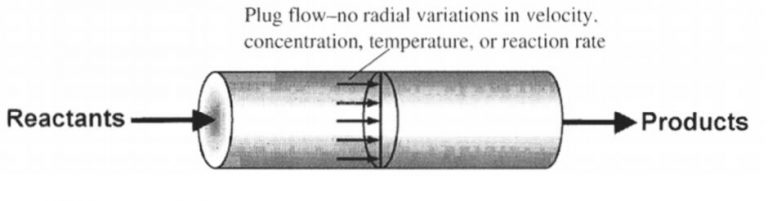
\includegraphics[width=0.7\textwidth]{Figures/sample.jpeg}
    \caption{Sample figure.}
    \label{fig:reactor_scheme}
\end{figure}

\subsection{PDE Representation of Delay Term}

One effective method for addressing delay in systems is to represent the delay using an alternative transport partial differential equation (PDE). This approach is particularly advantageous when the problem already involves similar forms of PDEs, as is the case in the current study. To specifically address the delay in the system under consideration, the state variable $c(\zeta, t)$ is expanded into a vector of functions $x(\zeta, t) \equiv [x_1(\zeta, t), x_2(\zeta, t)]^T$, where $x_1(\zeta, t)$ represents the concentration within the reactor, and $x_2(\zeta, t)$ is introduced as a new state variable to account for the concentration along the recycle stream. The delay is thus modeled as a pure transport process, wherein the first state $x_1(\zeta, t)$ is transported from the reactor outlet to the inlet, experiencing a delay of $\tau$ time units while in the recycle stream. As a result, Equations~\ref{eq:PDE_original_model}~and~\ref{eq:BC} may be re-formulated as follows:

\begin{align}
    \partial_t 
    \begin{bmatrix}
        x_1(\zeta, t) \\ x_2(\zeta,t)
    \end{bmatrix}
    =
    \begin{bmatrix}
        D \partial_{\zeta \zeta} - v \partial_\zeta + k_r && 0 \\
        0 && -\frac{1}{\tau} \partial_\zeta
    \end{bmatrix}
    \begin{bmatrix}
        x_1(\zeta, t) \\ x_2(\zeta,t)
    \end{bmatrix}\\
\begin{cases}
    D \partial_\zeta x_1(0, t) - v x_1(0, t) = -v \left[ R x_2(0, t) + (1-R) u(t) \right] \\
    \partial_\zeta x_1(1, t) = 0 \\
    x_1(1,t) = x_2(1,t) \\
    y(t) = x_1(1, t)
\end{cases}
\end{align}

With all state variables now expressed explicitly at a specific time instance $t$—in contrast to the previous representation where states at $t$ were directly involved with states at $(t-\tau)$—the system can be described in the standard state-space form of an infinite-dimensional linear time-invariant (LTI) system as $\dot{x} = \mathfrak{A} x$. Here, the state $x(\zeta, t) = [x_1(\zeta, t), x_2(\zeta, t)]^T$ is a vector of functions, and $\mathfrak{A}$ is a linear operator $\mathcal{L}(X)$ acting on a Hilbert space $X: L^2[0,1] \times L^2[0,1]$. The operator $\mathfrak{A}$ and its domain are defined in detail as shown in Equation~\ref{eq:operator_A}:

\begin{equation} \label{eq:operator_A}
    \begin{aligned}
        \mathfrak{A} \equiv&
        \begin{bmatrix}
            D \partial_{\zeta \zeta} - v \partial_\zeta + k_r & 0 \\
            0 & \frac{1}{\tau} \partial_\zeta
        \end{bmatrix}\\
        D(\mathfrak{A}) =& \Bigl\{ x = [x_1, x_2]^T \in X:
        x(\zeta), \partial_\zeta x(\zeta), \partial_{\zeta \zeta} x(\zeta) \quad \mathrm{a.c.},\\
        &D \partial_\zeta x_1(0) - v x_1(0) = -v \left[ R x_2(0) + (1-R) u \right],\\
        &\partial_\zeta x_1(1) = 0,
        x_1(1) = x_2(1) \Bigr\}
    \end{aligned}
\end{equation}

\subsection{Adjoint Operator}

The adjoint operator $\mathfrak{A}^*$ plays a critical role in analyzing the spectral properties of the system. It is obtained in Equation~\ref{eq:adjoint_A}:

\begin{equation} \label{eq:adjoint_A}
    \begin{aligned}
        \langle \mathfrak{A} \phi, \psi\rangle  = \langle \phi, {\mathfrak{A}}^{*} \psi\rangle  &\Rightarrow \\
        {\mathfrak{A}}^{*} =&
        \begin{bmatrix}
            D \partial_{\zeta \zeta} + v \partial_\zeta +k_r & 0\\
            0 & -\frac{1}{\tau} \partial_\zeta
        \end{bmatrix}\\
        D(\mathfrak{A}^*) =& \Bigl\{ y = [y_1, y_2]^T \in Y:
        y(\zeta), \partial_\zeta y(\zeta), \partial_{\zeta \zeta} y(\zeta) \quad \mathrm{a.c.},\\
        &D \partial_\zeta y_1(1) + v y_1(1) = \frac{1}{\tau} y_2(1) \\
        &R v y_1(0) = \frac{1}{\tau} y_2(0) \\
        &\partial_\zeta y_1(0) = 0 \Bigr\}
    \end{aligned}
\end{equation}

where $\phi_i(\zeta) = [\phi_{i,1}(\zeta), \phi_{i,2}(\zeta)]^T$ and $\psi_i(\zeta) = [\psi_{i,1}(\zeta), \psi_{i,2}(\zeta)]^T$ are the eigenfunction of $\mathfrak{A}$ and $\mathfrak{A}^*$, respectively. Given that $\mathfrak{A}$ is not self-adjoint (i.e., $\mathfrak{A} \neq \mathfrak{A}^*$), their combined eigenmodes may still form a bi-orthonormal basis, typical of a Riesz-spectral operator \autocite{curtainbook}. Therefore their spectral properties must be determined by solving their characteristic equations.

\subsection{Eigenvalue Problem}

The eigenvalue problem\autocite{pdebook} for $\mathfrak{A}$ is formulated as:

\begin{equation} \label{eq:eig_prob}
        \mathfrak{A} \phi_i(\zeta) = \lambda_i \phi_i(\zeta)
\end{equation}

% \begin{equation} \label{eq:eigval_calc_1}
%     \begin{aligned}
%         &\begin{cases}
%             &\lambda \phi_1 = D \frac{d^2 \phi_1}{d \zeta ^2}  - v \frac{d \phi_1}{d \zeta} + k \phi_1 \\
%             &\lambda \phi_2 = \frac{1}{\tau} \frac{d \phi_2}{d \zeta}
%         \end{cases} \\ B.C. &\begin{cases}
%             &D \left. \frac{d \phi_1}{d \zeta} \right|_{\zeta=0} - v \left. \phi_1 \right|_{\zeta=0} = - R v \left. \phi_2 \right|_{\zeta=0} \\
%             &\left. \phi_1 \right|_{\zeta=1} = 0 \\
%             &\left. \phi_1 \right|_{\zeta=1} = \left. \phi_2 \right|_{\zeta=1}
%         \end{cases}
%     \end{aligned}
% \end{equation}

where $\lambda_i \in \mathbb{C}$ is the $i^{\text{th}}$ eigenvalue. To obtain the characteristic equation, the system of PDEs shall be reduced to the ODE system in Equation~\ref{eq:eigval_calc_2} $\forall i \geq 0$:

\begin{equation} \label{eq:eigval_calc_2}
    \begin{aligned}
        \partial_\zeta \begin{bmatrix}
            \phi_1 \\ \partial_\zeta \phi_1 \\ \phi_2
        \end{bmatrix} = \begin{bmatrix}
            0 & 1 & 0 \\
            \frac{\lambda-k_r}{D} & \frac{v}{D} & 0 \\
            0 & 0 & \tau \lambda 
        \end{bmatrix} \begin{bmatrix}
            \phi_1 \\ \partial_\zeta \phi_1 \\ \phi_2
        \end{bmatrix}
    \end{aligned}
\end{equation}

which is in the form of $ \tilde{\phi}_\zeta  = \tilde{\mathfrak{A}} \tilde{\phi}$, with the solution stated in Equation~\ref{eq:eigval_calc_3}:

\begin{equation} \label{eq:eigval_calc_3}
    \begin{bmatrix}
        \phi_1 \\ \partial_\zeta \phi_1 \\ \phi_2
    \end{bmatrix}_{\zeta=1} = \begin{bmatrix}
        \Lambda_{1,1} & \Lambda_{1,2} & \Lambda_{1,3} \\
        \Lambda_{2,1} & \Lambda_{2,2} & \Lambda_{2,3} \\
        \Lambda_{3,1} & \Lambda_{3,2} & \Lambda_{3,3}
    \end{bmatrix} \begin{bmatrix}
        \phi_1 \\ \partial_\zeta \phi_1 \\ \phi_2
    \end{bmatrix}_{\zeta=0}
\end{equation}

where the matrix $\Lambda_{(i,j)}$ is defined as $e^{\tilde{\mathfrak{A}}}$. By applying the boundary conditions to Equation~\ref{eq:eigval_calc_3}, the algebraic system of equations in Equation~\ref{eq:eigval_calc_4} is obtained:

\begin{equation} \label{eq:eigval_calc_4}
    \begin{bmatrix}
        -v & D & Rv \\
        \Lambda_{2,1} & \Lambda_{2,2} & \Lambda_{2,3} \\
        (\Lambda_{1,1} - \Lambda_{3,1}) & (\Lambda_{1,2} - \Lambda_{3,2}) & (\Lambda_{1,3} - \Lambda_{3,3})
    \end{bmatrix} \begin{bmatrix}
        \phi_1 \\ \partial_\zeta \phi_1 \\ \phi_2
    \end{bmatrix}_{\zeta=0} = \tilde{\Lambda} \tilde{\phi}_{\zeta = 0} = 0
\end{equation}

where $\tilde{\Lambda}$ is defined as the square matrix shown in Equation~\ref{eq:eigval_calc_4}. Equation~\ref{eq:eigval_calc_4} suggests that the matrix $\tilde{\Lambda}$ must be rank-deficient for appropriate values of $\lambda_i$. Attempts to analytically solve the characteristic equation $det(\tilde{\Lambda}) = 0$ has failed; therefore, it is solved numerically using the parameters in Table~\ref{tab:pars}. The resulting eigenvalue distribution is depicted in Figure~\ref{fig:eigval_dist} in the complex plane.

\begin{table}[ht]
    \centering
    \caption{Physical Parameters for the System}
    \label{tab:pars}
    \begin{tabular}{|c|c|c|c|}
    \hline
    \textbf{Parameter}        & \textbf{Symbol} & \textbf{Value}     & \textbf{Unit}    \\ \hline
    Diffusivity               & $D$             & $2\times10^{-5}$   & ${m^2}/{s}$      \\ \hline
    Velocity                  & $v$             & $1\times10^{-2}$   & ${m}/{s}$        \\ \hline
    Reaction Constant         & $k_r$           & $1.5$              & $s^{-1}$         \\ \hline
    Recycle Residence Time    & $\tau$          & $80$               & $s$              \\ \hline
    Recycle Ratio             & $R$             & $0.3$              & $-$              \\ \hline
    \end{tabular}
\end{table}

\begin{figure}[ht]
    \centering
    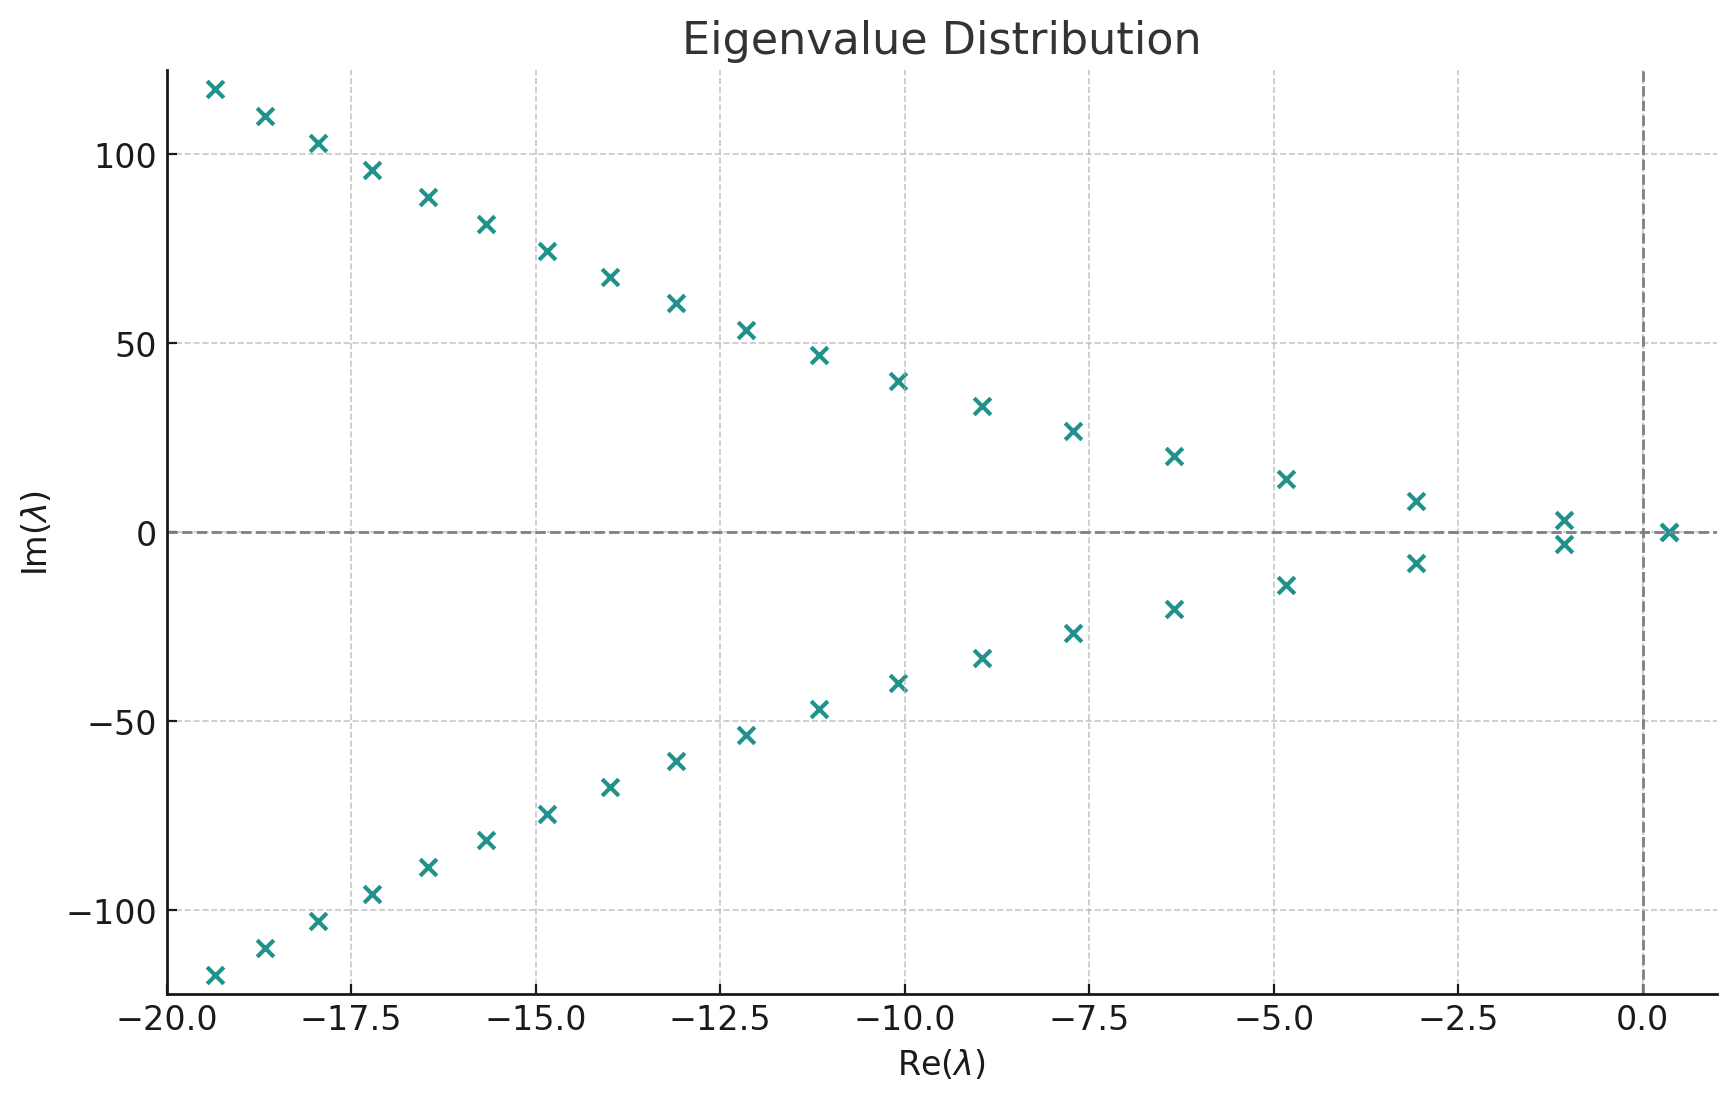
\includegraphics[width=0.7\textwidth]{Figures/eigval_dist_R_0.3.jpg}
    \caption{Eigenvalues of operator $\mathfrak{A}$ plotted on complex plane}
    \label{fig:eigval_dist}
\end{figure}

Following the same procedure for $\mathfrak{A}^*$ shows that the eigenvalues of $\mathfrak{A}$ match the ones of its adjoint, confirming that $\mathfrak{A}$ and $\mathfrak{A}^*$ form a bi-orthogonal basis according to Equation~\ref{eq:biorth}:

\begin{equation} \label{eq:biorth}
    \begin{aligned}
        &\langle \mathfrak{A} \phi_i, \psi_j \rangle = \langle \lambda_i \phi_i, \psi_j \rangle = \lambda_i \langle \phi_i, \psi_j \rangle \\
        \text{L.H.S.} = &\langle \phi_i, \mathfrak{A}^* \psi_j \rangle = \langle \phi_i, \lambda_j^* \psi_j \rangle = \overline{\lambda_j^*} \langle \phi_i, \psi_j \rangle \\
        &\lambda_i = \overline{\lambda_i^*} \Rightarrow \langle \phi_i, \psi_j \rangle = \delta_{ij}
    \end{aligned}
\end{equation}

The eigenfunctions $\{ \phi_i(\zeta), \psi_i(\zeta) \}$ (for $\mathfrak{A}$ and $\mathfrak{A}^*$, respectively) may be obtained following the calculation of eigenvalues. The first 3 eigenfunctions are plotted in Figure~\ref{fig:eigfun}. 

\begin{figure}[ht]
    \centering
    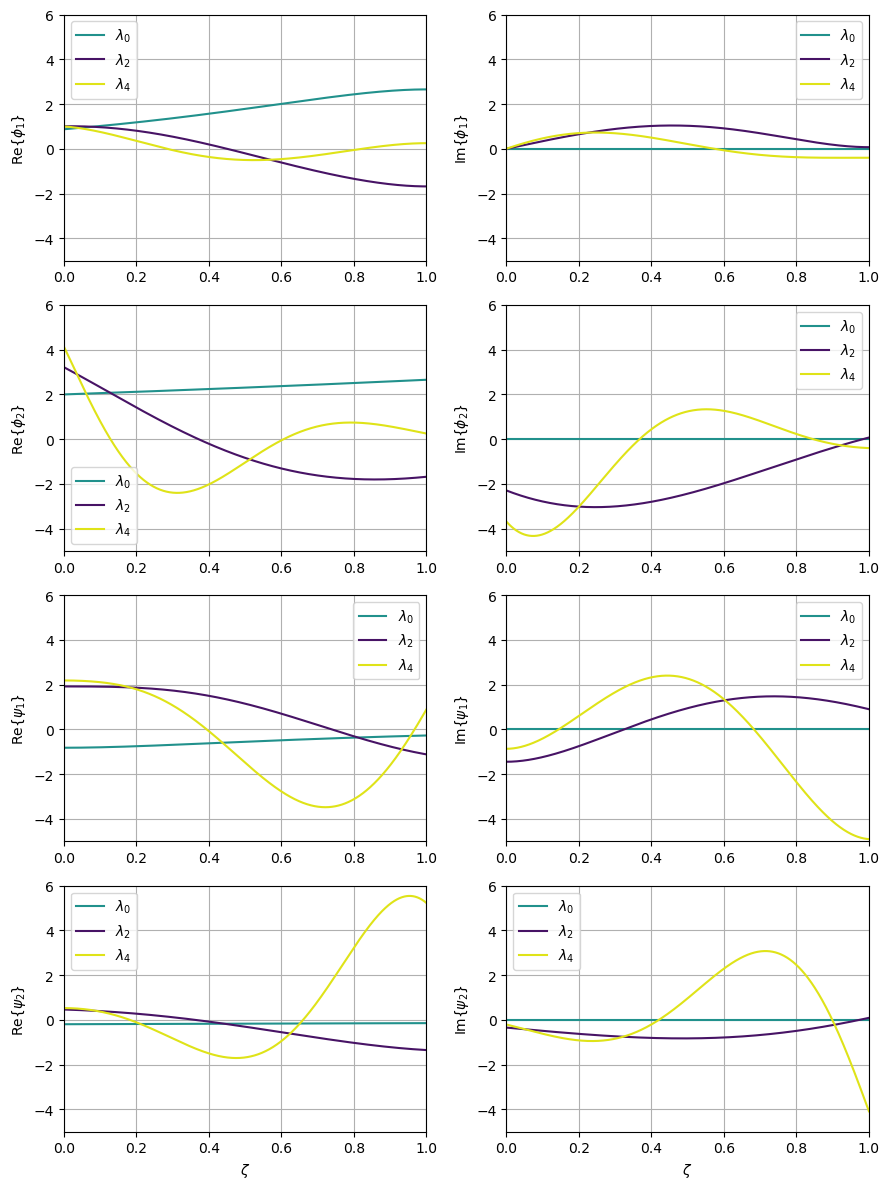
\includegraphics[width=0.7\textwidth]{Figures/eigfuns.png}
    \caption{First few eigenmodes of $\mathfrak{A}$ and $\mathfrak{A}^*$}
    \label{fig:eigfun}
\end{figure}

  
  \section{LINEAR QUADRATIC REGULATOR DESIGN} \label{sec:control}

\subsection{Full-state feedback regulator} \label{sec:fullstate_design}

The bi-orthogonal basis generated by the Riesz-spectral operator $\mathfrak{A}$ in the LTI system $\mathbf{\Sigma(\mathfrak{A},\mathfrak{B},\mathfrak{C},-)}$ provides the foundation for solving the Operator Riccati Equation (ORE), a crucial step in the design of a Linear Quadratic Regulator (LQR). The objective is to derive a feedback control law that minimizes the infinite-time cost function, as defined in Equation~\ref{eq:cost_fun}, with $\mathfrak{Q}$ and $\mathfrak{R}$ being self-adjoint coercive operators that penalize state deviations and control actions, respectively.

\begin{equation} \label{eq:cost_fun}
    J(x_0, u) = \int_{t=0}^{\infty} \langle \bm{x}(s), \mathfrak{Q} \bm{x}(s)\rangle + \langle u(s), \mathfrak{R} u(s)\rangle ds
\end{equation}

\subsubsection{Operator Riccati equation}

The LQR problem is solved by finding the unique positive semi-definite operator $\mathbf{\Pi}$, which satisfies the ORE presented in Equation~\ref{eq:ORE_1}. This operator is then used to compute the feedback gain that ensures optimal control of the system.

\begin{equation} \label{eq:ORE_1}
    \langle \mathfrak{A}^* \mathbf{\Pi} \bm{x}, \bm{y}\rangle + \langle \mathbf{\Pi} \mathfrak{A} \bm{x}, \bm{y} \rangle - \langle \mathbf{\Pi} \mathfrak{B} \mathfrak{R}^{-1} \mathfrak{B}^* \mathbf{\Pi} \bm{x}, \bm{y}\rangle + \langle \mathfrak{Q} \bm{x}, \bm{y}\rangle = 0
\end{equation}

Given that the solution to the ORE is unique for any set of functions in the domain of operator $\mathfrak{A}$, we can select $\bm{x} = \bm{\phi_m}$ and $\bm{y} = \bm{\phi_n}$, i.e. the eigenfunctions of $\mathfrak{A}$. Applying this choice, and noting that $\mathbf{\Pi}$ is self-adjoint, leads to the simplified Equation~\ref{eq:ORE_2}.

\begin{equation} \label{eq:ORE_2}
    \langle \mathbf{\Pi} \bm{\phi_m}, \mathfrak{A} \bm{\phi_n} \rangle
    + \langle \mathfrak{A} \bm{\phi_m}, \mathbf{\Pi} \bm{\phi_n} \rangle
    - \mathfrak{R}^{-1} \langle \mathfrak{B}^* \mathbf{\Pi} \bm{\phi_m}, \mathfrak{B}^* \mathbf{\Pi} \bm{\phi_n} \rangle 
    + \langle \mathfrak{Q} \bm{\phi_m}, \bm{\phi_n} \rangle = 0
\end{equation}

To ensure that the domain and range of $\mathbf{\Pi}$ match those of $\mathfrak{A}$ and $\mathfrak{A}^*$, respectively, $\mathbf{\Pi}$ can be expressed as an infinite series, as shown in Equation~\ref{eq:P}. The coefficients $p_{i,j}$ can be interpreted as elements of an infinite-dimensional matrix $\tilde{P}$, which represents the operator $\mathbf{\Pi}$. This forms the first step in converting the ORE to the corresponding Matrix Riccati Equation (MRE).

\begin{equation} \label{eq:P}
    \mathbf{\Pi} x \equiv \sum_{i=1}^{\infty}\sum_{j=1}^{\infty} p_{i,j} \langle \bm{x}, \bm{\psi_j} \rangle \bm{\psi_i} \qquad
    \forall {i,j}: \quad p_{i,j} \in \mathbb{C}
\end{equation}

\subsubsection{Obtaining $\mathfrak{B}$ and $\mathfrak{B}^*$}

Before further simplifying the ORE, it is essential to define the operators $\mathfrak{B}$ and $\mathfrak{B}^*$. Given the boundary-control nature of the system as seen in Equation~\ref{eq:BC}, $\mathfrak{B}$ is defined to properly project the control input $u \in \mathbb{R}^1$ onto the state space $X: L^2[0,1] \times L^2[0,1]$, as outlined in Equation~\ref{eq:B}.

\begin{equation} \label{eq:B}
    \mathfrak{B} u \equiv v(1-R)
    \begin{bmatrix}
        \delta(\zeta) \\ 0
    \end{bmatrix} \cdot u
\end{equation}

The adjoint operator $\mathfrak{B}^*$ is obtained by leveraging the properties of $\mathfrak{A}$ and $\mathfrak{A}^*$, i.e. their expressions as well as their domains (as shown in Equations~\ref{eq:operator_A}~and~\ref{eq:adjoint_A}), after applying integration by parts to the result of the inner products, as summarized in Equation~\ref{eq:B*}.

\begin{equation} \label{eq:B*}
    \begin{aligned}
        \langle \mathfrak{A} \bm{x} + \mathfrak{B} u, \bm{y} \rangle
        &= \langle \mathfrak{A} \bm{x}, \bm{y} \rangle
        + \langle \mathfrak{B} u, \bm{y} \rangle
        = \langle \bm{x}, \mathfrak{A}^* \bm{y}\rangle
        + \langle u, \mathfrak{B}^* \bm{y} \rangle \\
        \langle u, \mathfrak{B}^* \bm{y} \rangle
        &= \langle \mathfrak{A} \bm{x} + \mathfrak{B} u, \bm{y} \rangle
        - \langle \bm{x}, \mathfrak{A}^* \bm{y}\rangle
        \Rightarrow \hdots \\ \Rightarrow \mathfrak{B}^* (\cdot) &= \Bigl[ v(1-R) \int_0^1 \delta(\zeta) (\cdot) d\zeta \quad , \quad 0 \Bigr]
    \end{aligned}
\end{equation}

\subsubsection{Matrix Riccati equation}

Using the expression for $\mathbf{\Pi}$ in Equation~\ref{eq:P}, along with the derived $\mathfrak{B}^*$ from Equation~\ref{eq:B*}, and the eigenvalue problem $\mathfrak{A}\bm{\phi_i} = \lambda_i \bm{\phi_i}$, the ORE can be reformulated as the Matrix Riccati Equation (MRE) shown in Equation~\ref{eq:MRE}. Here, $\gamma_i \equiv v(1-R) \left. \psi_{1}^{(i)} \right|_{\zeta = 0}$, and $q_{m,n} = \langle \mathfrak{Q} \bm{\phi_m}, \bm{\phi_n} \rangle$.

\begin{equation}\label{eq:MRE}
    p_{n,m} (\lambda_m + \overline{\lambda_n})
    - \mathfrak{R}^{-1} \langle \sum_{i=1}^\infty p_{i,m} \gamma_i, \sum_{i=1}^\infty p_{i,n} \gamma_i \rangle
    + q_{m,n} = 0
\end{equation}

Due to the infinite-dimensional nature of $\tilde{P}$, a numerical solution is impractical. This challenge is addressed by selecting the first $N$ eigenmodes of the system as its dominant modes. This means truncating the infinite sums in the MRE and reducing the infinite-dimensional system to a finite set of nonlinear algebraic equations that can be solved to obtain an equivalent $N \times N$ matrix $P$, i.e. a truncated approximation of matrix $\tilde{P}$. The optimal full-state feedback gain is then calculated using Equation~\ref{eq:fullstate_gain}, ensuring closed-loop stability.

\begin{equation} \label{eq:fullstate_gain}
    \begin{aligned}
        u(t) &= - \langle \bm{K}(\zeta), \bm{x}(\zeta, t) \rangle = - \mathfrak{B}^* \mathbf{\Pi} \bm{x}(\zeta, t) \\
        &= - \sum_{i=1}^N\sum_{j=1}^N p_{i,j} \langle \bm{x}(\zeta, t), \bm{\psi_j}(\zeta) \rangle \gamma_i \\
        &= - \sum_{i=1}^N\sum_{j=1}^N p_{i,j} \gamma_i \int_0^1 \bm{x}(\zeta, t) \cdot \overline{\bm{\psi_j}}(\zeta) d\zeta \\
        &= - \int_0^1 \sum_{i=1}^N\sum_{j=1}^N p_{i,j} \gamma_i \overline{\bm{\psi_j}}(\zeta) \cdot \bm{x}(\zeta, t) d\zeta \\
        \Rightarrow \bm{K}(\zeta) &\equiv \sum_{i=1}^N\sum_{j=1}^N p_{i,j} \gamma_i \overline{\bm{\psi_j}}(\zeta)
    \end{aligned}
\end{equation}

The computed gain is a function of space and is calculated offline. The control action at any given time instance is the inner product of this gain with the current state of the system, thus justifying the term ``full-state'' feedback. The dynamics of the resulting closed-loop full-state feedback system may be described by the state-space representation shown in Equation~\ref{eq:fullstate_ss}.

\begin{equation}
    \begin{aligned} \label{eq:fullstate_ss}
        \dot{x}(\zeta, t) &= \mathfrak{A} \bm{x}(\zeta, t) + \mathfrak{B} u(t) \\
        &= (\mathfrak{A} - \mathfrak{B} \bm{K}) \, \bm{x}(\zeta, t) \\
        &= \mathfrak{A}_{reg} \, \bm{x}(\zeta, t)
    \end{aligned}
\end{equation}

By selecting $\mathfrak{Q} = 0.05$ as a constant function over $\zeta = [0,1]$, and $\mathfrak{R} = 50$, the full-state feedback gain is obtained and represented in Figure~\ref{fig:k_modes}. The obtained gains are used to design the optimal full-state feedback regulator to stabilize the control system. A block diagram representation of the full-state feedback control system is shown in Figure~\ref{fig:block_diagram}.

\begin{figure}[!htbp]
    \centering
    \begin{subfigure}[b]{0.45\textwidth}
        \centering
        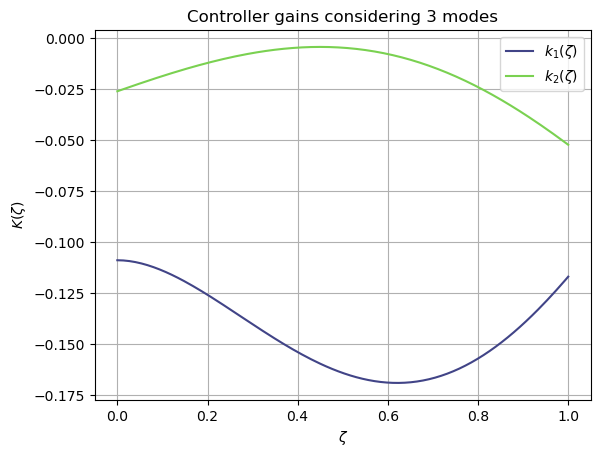
\includegraphics[width=\textwidth]{Figures/k_3.png}
        \caption{$N = 3$}
        \label{fig:k_3}
    \end{subfigure}
    \hfill
    \begin{subfigure}[b]{0.45\textwidth}
        \centering
        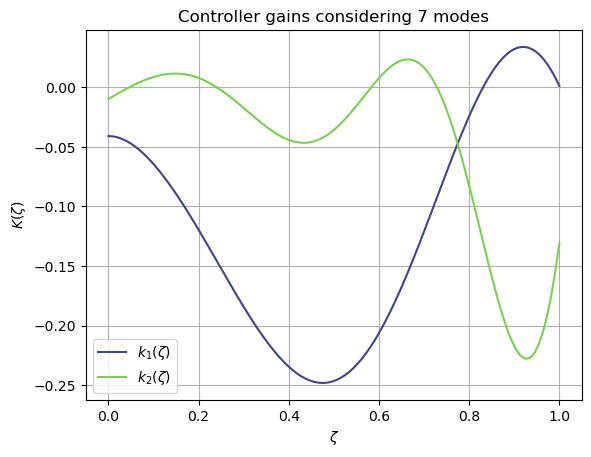
\includegraphics[width=\textwidth]{Figures/k_7.png}
        \caption{$N = 7$}
        \label{fig:k_7}
    \end{subfigure}
    \caption{Full-state feedback gain $\bm{K}(\zeta)$ utilizing the first $N$ modes of the system given by Equation~(\ref{eq:fullstate_gain}).}
    \label{fig:k_modes}
\end{figure}

\begin{figure}[!htbp]
    \centering
    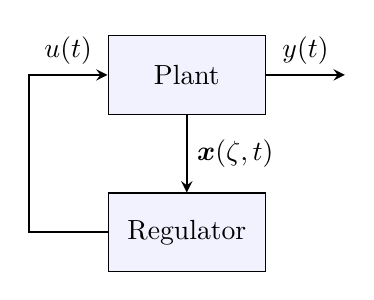
\begin{tikzpicture}[node distance=2cm]
        \node (plant) [block_1] {Plant};
        \node (regulator) [block_1, below of=plant] {Regulator};
        \draw [arrow] (plant.south) -- node[midway, right] {$\bm{x}(\zeta,t)$} (regulator.north);
        \draw [arrow] (regulator.west) -- ++(-1,0) |- node[near end, above] {$u(t)$} (plant.west);
        \draw [arrow] (plant.east) -- node[midway, above] {$y(t)$} ++(1,0);
    \end{tikzpicture}
    \caption{Block diagram representation of the optimal full-state feedback control system.}
    \label{fig:block_diagram}
\end{figure}

\subsection{Output feedback compensator} \label{sec:output_design}

Thus far, the optimal regulator is designed under the assumption that it has full access to the system's states. However, this assumption is not feasible in realistic applications. To address this, an observer is introduced to estimate and reconstruct the states by measuring the system's output in real time, and providing the regulator with the reconstructed states to further stabilize the system. The output, in this context, is taken as the concentration at the reactor outlet, as defined in Equation~\ref{eq:BC}. This leads to the definition of the output operator $\mathfrak{C}$ in the linear time-invariant (LTI) system $\mathbf{\Sigma(\mathfrak{A},\mathfrak{B},\mathfrak{C},-)}$, which is subsequently used to determine the observer gain, $\bm{L}(\zeta)$. The formulation is shown in Equation~\ref{eq:C}:

\begin{equation} \label{eq:C}
    \mathfrak{C} \equiv \begin{bmatrix}
        \int_0^1 \delta(\zeta-1) ( \cdot ) d\zeta \quad , \quad 0
    \end{bmatrix}
\end{equation}

where $\delta(\zeta)$ denotes the Dirac delta function. Regarding the choice of observer, Luenberger-based observers are well-suited for infinite-dimensional systems when the system parameters are perfectly known \autocite{ali2015reviewobserver}. Among the various methods to compute the gain for this class of observers, pole-placement is a solid, straightforward, and reliable approach for state reconstruction. To ensure that the state reconstruction dynamics converge more quickly than the regulation dynamics, the poles of the observer-based controller are placed to the left of the poles of the full-state feedback controller. This practice is common in the design of observer-based controllers for infinite-dimensional systems \autocite{morrisbook}. The observer gain in Figure~\ref{fig:L_modes} is obtained by limiting the eigenmodes of the observer-based controller to have real parts that are at least 3 times more negative than the real part of the dominant eigenmodes of the full-state feedback system. This is done for the case where the first 7 modes of the system are considered for designing the controller. The first few eigenvalues of the observer-based controller and the full-state feedback controller, along with the eigenvalues of the open-loop system are shown in Figure~\ref{fig:eigs} to demonstrate the pole placement strategy explained above. It can be confirmed that both control systems have eigenvalues with negative real parts, ensuring stability. Note that the eigenvalues of both control systems are identical after the 7th mode, as the real parts of these eigenvalues are already sufficiently negative.

\begin{figure}[!htbp]
    \centering
    \includesvg[inkscapelatex=false, width=0.5\textwidth, keepaspectratio]{Figures/L.svg}
    \caption{Observer gain $\bm{L}(\zeta)$.}
    \label{fig:L_modes}
\end{figure}

\begin{figure}[!htbp]
    \centering
    \includesvg[inkscapelatex=false, width=0.5\textwidth, keepaspectratio]{Figures/pole_placement.svg}
    \caption{Eigenvalues of the observer-based controller, full-state feedback controller, and open-loop system.}
    \label{fig:eigs}
\end{figure}

The dynamics of the augmented observer-controller system are described by the state-space representation shown in Equation~\ref{eq:observer_ss}, where $\hat{\bm{x}}(\zeta, t)$ and $\bm{e}(\zeta, t)$ refer to the estimated state and the state estimation error, respectively. A block diagram representation of the output feedback control system is also shown in Figure~\ref{fig:block_diagram_observer}.

\begin{figure}[!htbp]
    \centering
    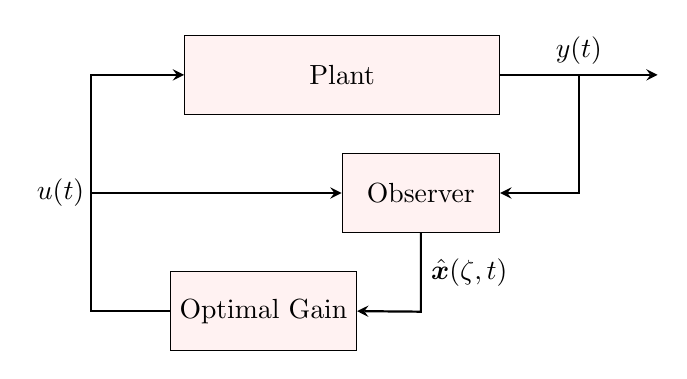
\begin{tikzpicture}[node distance=2cm]
        \node (plant) [block_2, minimum width=4cm] {Plant};
        \node (regulator) [block_2, below of=plant, xshift=-1cm, yshift=-1cm] {Optimal Gain};
        \node (observer) [block_2, below of=plant, xshift=1cm, yshift=0.5cm] {Observer};
        \draw [arrow] (plant.east) -- node[midway, above] {$y(t)$} ++(2,0);
        \draw [arrow] (plant.east) ++(1,0) |- (observer.east);
        \draw [arrow] (observer.south) -- ++(0,-1) node[midway, right] {$\hat{\bm{x}}(\zeta,t)$} -- (regulator.east);    
        \draw [arrow] (regulator.west) -- ++(-1,0) |- (plant.west);
        \draw [arrow] (regulator.west) ++(-1,1.5) coordinate(start) -- node[near start, left, xshift=-0.75cm] {$u(t)$} (observer.west);
    \end{tikzpicture}
    \caption{Block diagram representation of the observer-based output feedback control system.}
    \label{fig:block_diagram_observer}
\end{figure}

\begin{equation}
    \begin{aligned} \label{eq:observer_ss}
        \left[\begin{array}{c}
            \dot{\bm{x}}(\zeta,t) \\ \hline \dot{\hat{\bm{x}}}(\zeta,t)
        \end{array}\right] &= 
        \left[
            \begin{array}{c|c}
                \mathfrak{A} & -\mathfrak{B} \bm{K} \\ \hline
                \bm{L} \mathfrak{C} & \mathfrak{A} - \mathfrak{B} \bm{K} - \bm{L} \mathfrak{C}
            \end{array}
        \right]
        \left[ \begin{array}{c}
            \bm{x}(\zeta,t) \\ \hline \hat{\bm{x}}(\zeta,t) \end{array}
            \right] \\
        \dot{\bm{e}}(\zeta,t) &= \left[ \dot{\bm{x}}(\zeta,t) - \dot{\hat{\bm{x}}}(\zeta,t) \right] \\
        &= (\mathfrak{A} - \bm{L} \mathfrak{C}) \, \bm{e}(\zeta,t) \\
        &= \mathfrak{A}_{est} \, \bm{e}(\zeta,t)
    \end{aligned}
\end{equation}

    
  \section{RESULTS AND DISCUSSION} \label{sec:results}

The obtained controller strategies in the previous section are applied to a finite-difference method (FDM) representation of the system model to evaluate the system dynamics. The system model is discretized in space and time, and the resulting system of ordinary differential equations is solved using the \texttt{`solve\_ivp'} function in Python's \texttt{`SciPy'} library \autocite{2020SciPy}, which employs the adaptive Runge-Kutta method of order 5(4), \texttt{`RK45'}. Each state of the system is discretized in space using 100 grid points. The \texttt{`RK45'} method automatically adjusts time steps to balance accuracy and computational efficiency, with the solution being evaluated at specific points as required \autocite{RK45_1,RK45_2}. First, the unstable dynamics of the open-loop system is explored. Then two full-state feedback systems are compared with respect to number of eigenmodes used to obtain the optimal feedback gain. Finally, the performance of the proposed observer-based controller is evaluated and the state reconstruction error dynamics are analyzed.

\subsection{FDM representation of the open-loop system}

Zero-input response of the system is explored using the mentioned FDM setup to show the unstable dynamics of the model. The state profile versus time and space $x_1(\zeta,t)$, is illustrated in Figure~\ref{fig:3D_x1_openloop}. The goal is to stabilize the system using an optimal control strategy. The system is unstable as the result of the generation term in the model.

\begin{figure}[!htbp]
    \centering
    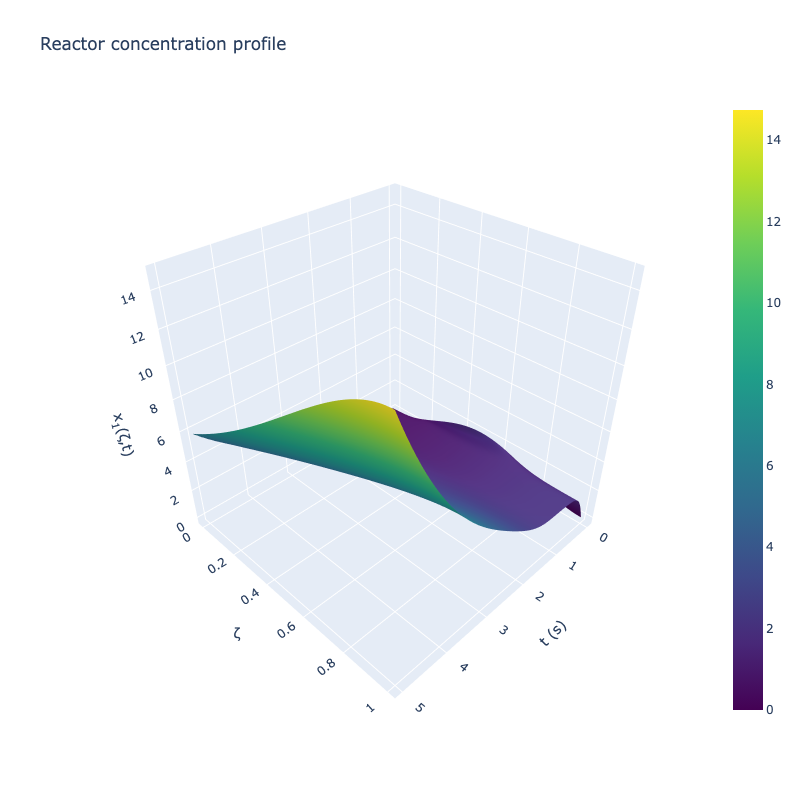
\includegraphics[width=0.8\textwidth,trim=0 0 100 0,clip]{Figures/3D_x1_openloop.png}
    \caption{Zero-input response of the unstable open-loop system as described by Equations~(\ref{eq:PDE_original_model})~and~(\ref{eq:BC}).}
    \label{fig:3D_x1_openloop}
\end{figure}

\subsection{Full-state feedback regulator FDM representation}


Next, the full-state feedback regulator is evaluated using the same FDM representation. Two configurations are compared where the optimal feedback gain is obtained using different number of eigenmodes: one with $N=3$ and another with $N=7$, according to Figure~\ref{fig:k_modes}. The state profile versus time and space is illustrated for both cases in Figure~\ref{fig:full_state_feedback}. 

\begin{figure}[!htbp]
    \centering
    \begin{subfigure}[b]{0.45\textwidth}
        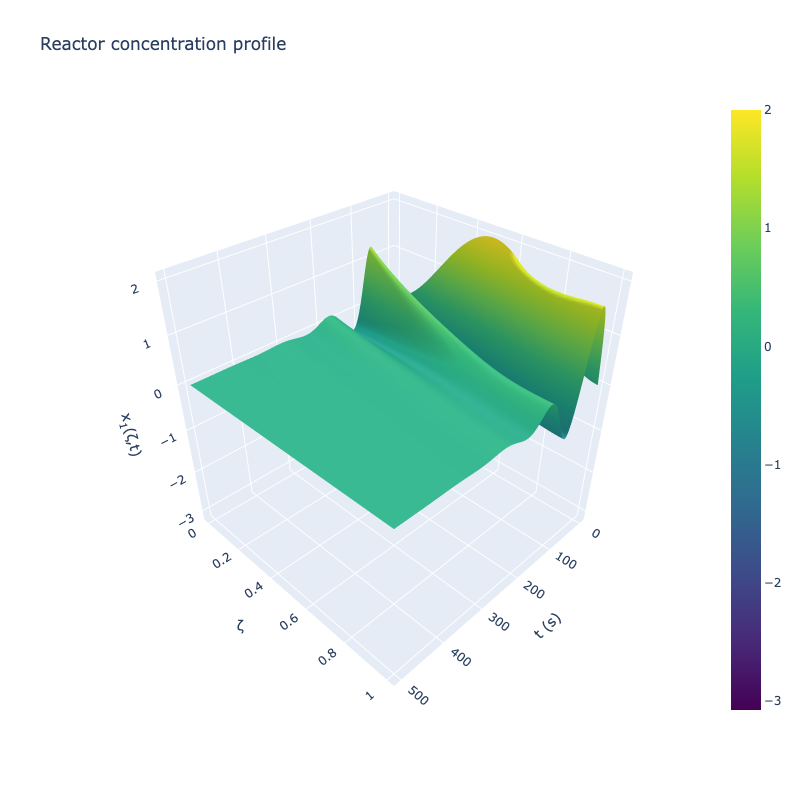
\includegraphics[width=\textwidth,trim=0 0 100 0,clip]{Figures/3D_x1_k3.png}
        \caption{$N=3$}
        \label{fig:3D_x1_k3}
    \end{subfigure}
    \hfill
    \begin{subfigure}[b]{0.45\textwidth}
        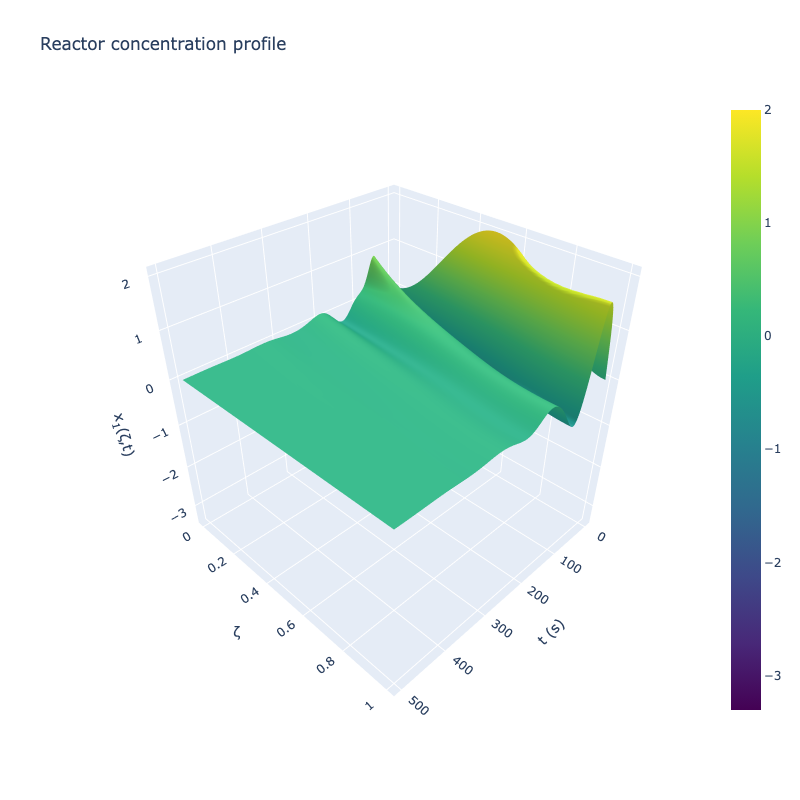
\includegraphics[width=\textwidth,trim=0 0 100 0,clip]{Figures/3D_x1_k7.png}
        \caption{$N=7$}
        \label{fig:3D_x1_k7}
    \end{subfigure}
    \caption{Input response of the system under full-state feedback control given by Equation~(\ref{eq:fullstate_ss}), utilizing the feedback gain obtained in Figure~\ref{fig:k_modes}.}
    \label{fig:full_state_feedback}
\end{figure}

Additionally, in order to offer a clearer representation of the state trajectory in time, spatial cross-sectional plots are provided in Figure~\ref{fig:2D_xt_k7} for the $N=7$ case at different lengths of the domain. The delay-imposing state, i.e. the concentration along the recycle stream $x_2(\zeta,t)$, is provided only in Figure~\ref{fig:2D_xt_k7} for the sake of conciseness.

\begin{figure}[!htbp]
    \centering
    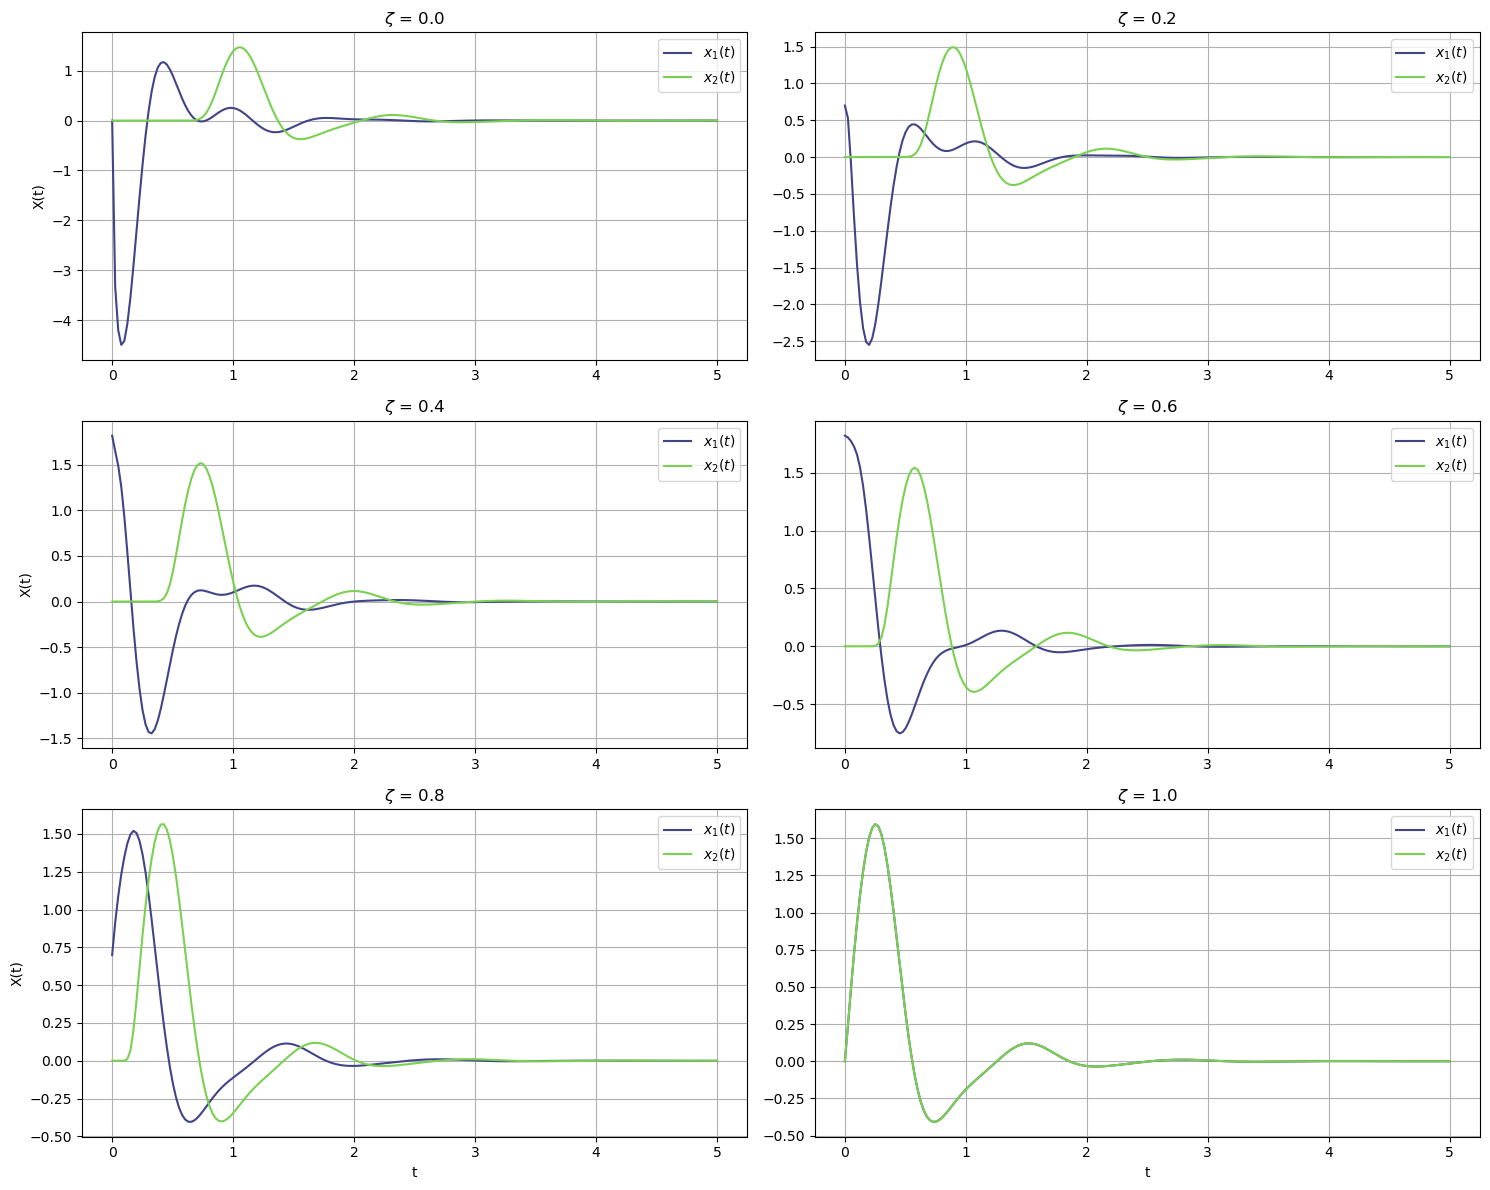
\includegraphics[width=0.8\textwidth]{Figures/2D_xt_k7.png}
    \caption{2D cross-section plots of the full-state feedback input response at various $\zeta$ positions, utilizing the feedback gain obtained in Figure~\ref{fig:k_7}.}
    \label{fig:2D_xt_k7}
\end{figure}

Both optimal feedback gains are able to successfully stabilize the system within finite time horizon. However, the case where more eigenmodes are considered in the controller design shows better performance in general. Sharing the same $\mathfrak{Q}$ and $\mathfrak{R}$ operators, the higher dimensional controller is able to stabilize the system quicker with lower cost function values in general.

\subsection{Observer-based regulator FDM representation}

Omitting the need to have full access to system states, the observer-based regulator is evaluated using the same FDM representation. The states reconstruction is done by applying the observer gain obtained in Figure~\ref{fig:L_modes} to the system output. The estimated states are now used with the previously obtained optimal feedback gain with $N=7$ eigenmodes to calculate the input. Similar to the previous case, the state profile $x_1(\zeta,t)$ is illustrated in Figure~\ref{fig:3D_x1_L_k7}, as well as cross-sectional plots for both states in Figure~\ref{fig:2D_xt_L_k7} for better visualization of state trajectories in time.

\begin{figure}[!htbp]
    \centering
    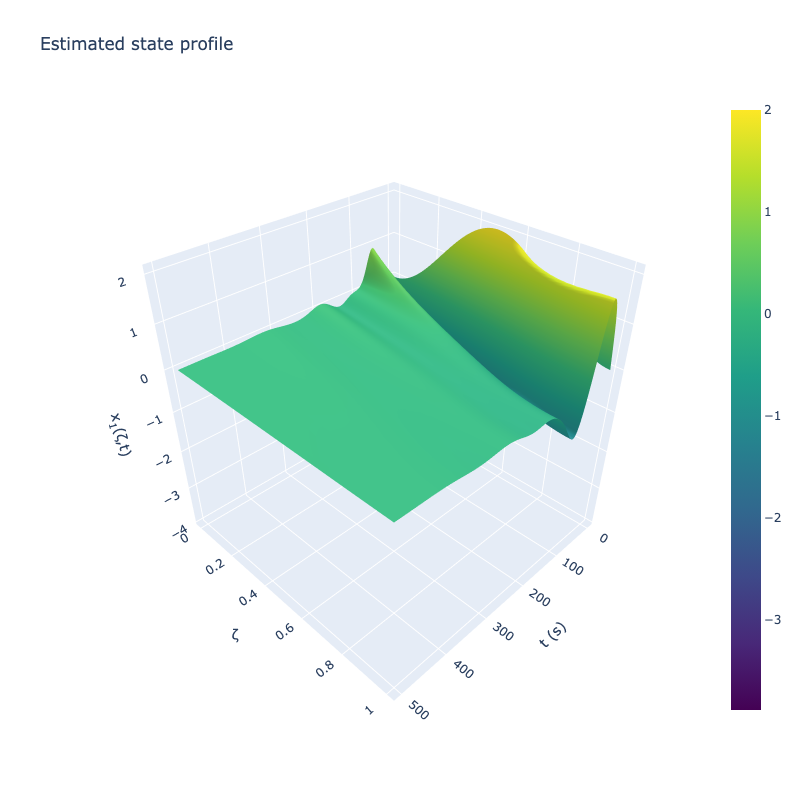
\includegraphics[width=0.8\textwidth,trim=0 0 100 0,clip]{Figures/3D_x1_L_k7.png}
    \caption{Input response of the system under observer-based output feedback control given by Equation~(\ref{eq:observer_ss}), utilizing the observer gain obtained in Figure~\ref{fig:L_modes} and the feedback gain obtained in Figure~\ref{fig:k_7}.}
    \label{fig:3D_x1_L_k7}
\end{figure}

\begin{figure}[!htbp]
    \centering
    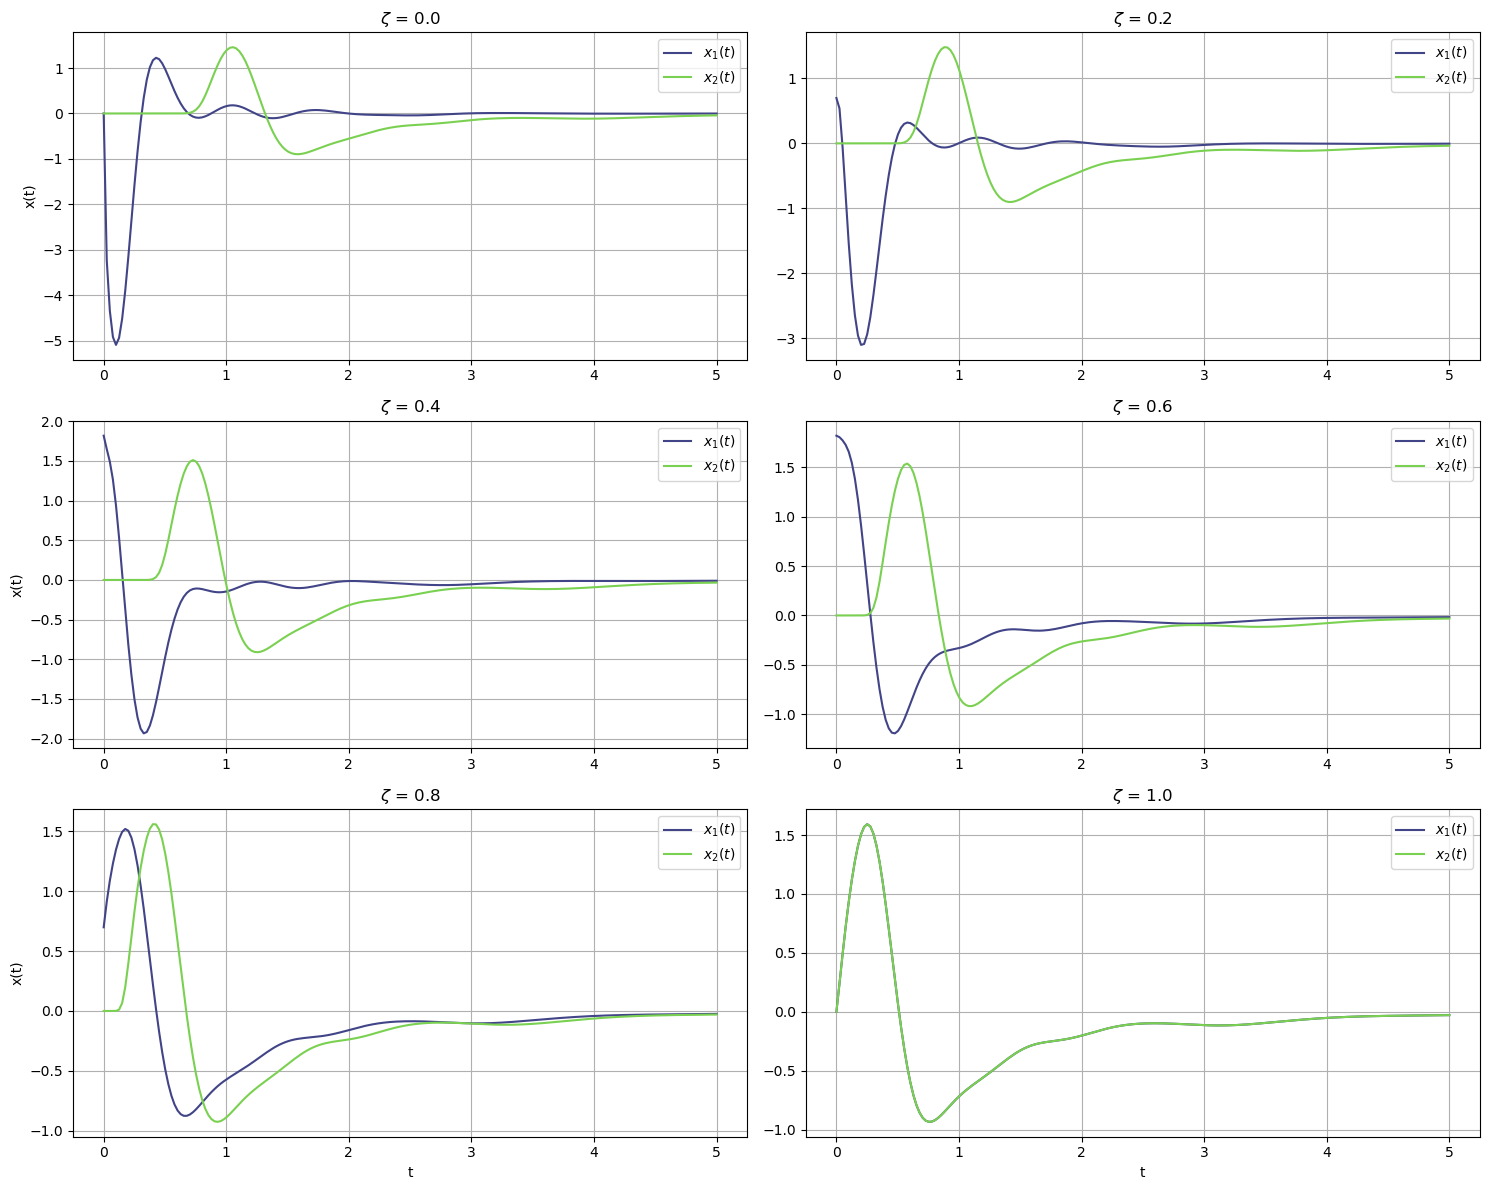
\includegraphics[width=0.8\textwidth]{Figures/2D_xt_L_k7.png}
    \caption{2D cross-section plots of the input response at various $\zeta$ positions, utilizing the observer gain obtained in Figure~\ref{fig:L_modes} and the feedback gain obtained in Figure~\ref{fig:k_7}.}
    \label{fig:2D_xt_L_k7}
\end{figure}

Last but not least, the state estimation error dynamics of the observer are plotted in Figures~\ref{fig:3D_e1_L_k7}~and~\ref{fig:2D_et_L_k7} to demonstrate the performance of the observer. The error dynamics are calculated as the squared difference between the true state and the estimated state at each grid point and time instance.

\begin{figure}[!htbp]
    \centering
    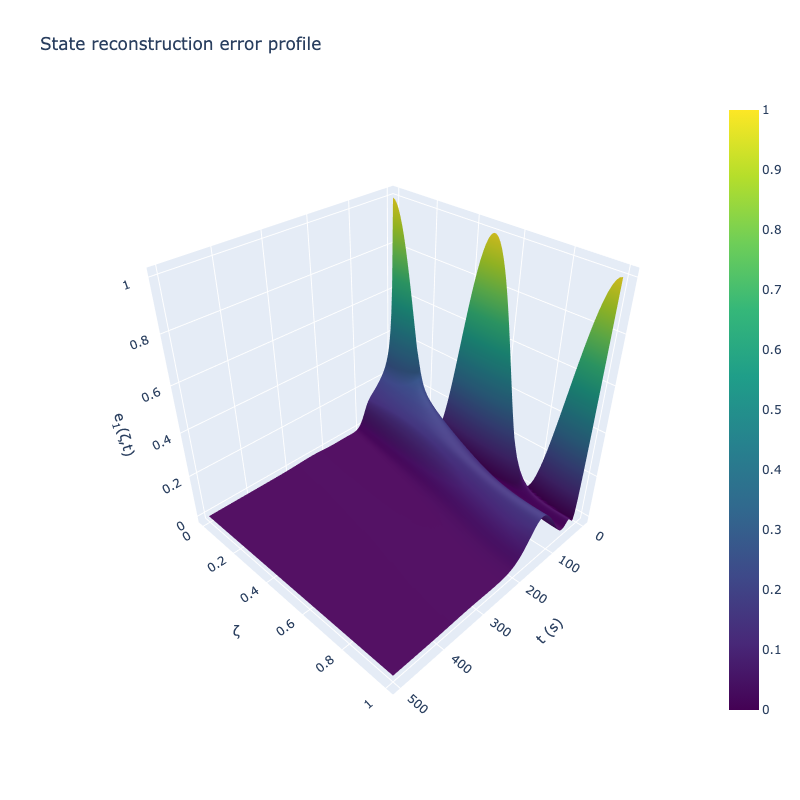
\includegraphics[width=0.8\textwidth,trim=0 0 100 0,clip]{Figures/3D_e1_L_k7.png}
    \caption{Error dynamics of the observer-based regulator utilizing the observer gain obtained in Figure~\ref{fig:L_modes} and the feedback gain obtained in Figure~\ref{fig:k_7}.}
    \label{fig:3D_e1_L_k7}
\end{figure}

\begin{figure}[!htbp]
    \centering
    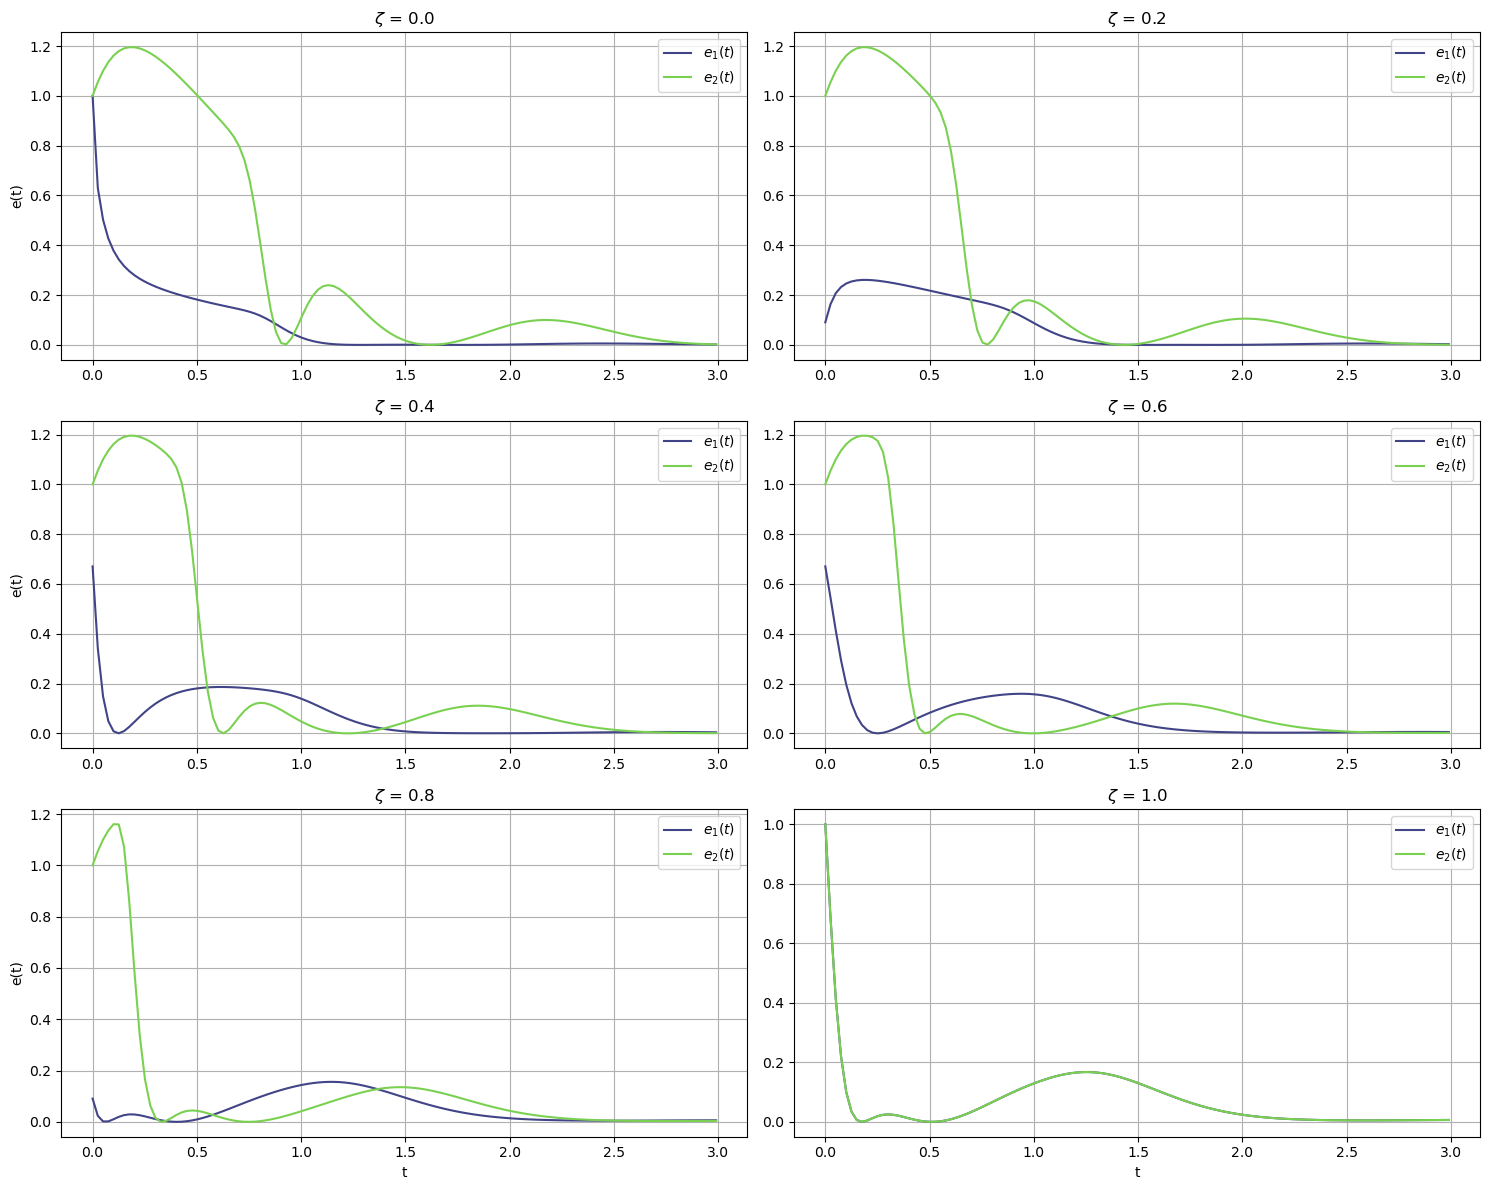
\includegraphics[width=0.8\textwidth]{Figures/2D_et_L_k7.png}
    \caption{2D cross-section plots of the error dynamics of the observer-based regulator at various $\zeta$ positions, utilizing the observer gain obtained in Figure~\ref{fig:L_modes} and the feedback gain obtained in Figure~\ref{fig:k_7}.}
    \label{fig:2D_et_L_k7}
\end{figure}

While the performance of the observer-based controller is slightly more sluggish compared to that of the full-state feedback regulator, it successfully stabilizes the system within a finite time horizon using only output measurements instead of full state information. In the absence of uncertainty in the system model, the observer gain can theoretically be designed so that the state estimation error converges to zero very fast compared to full-state feedback regulator dynamics. In practice, however, the observer gain is constrained by factors such as noise in the system output and plant-model mismatches. Despite these challenges, the proposed observer design mechanism achieves system stabilization with reasonable performance.

  \section{CONCLUSION}

The control of an axial tubular reactor equipped with recycle stream is addressed as a significant class of distributed parameter systems in chemical engineering industries. The notion of time delay introduced by the recycle process has not been adequately addressed in the literature despite being a common and intrinsic feature of such systems; introducing a rare example of state-delay in this field. By converting the notion of delay into an equivalent transport PDE, the DPS is formulated as a system of coupled parabolic and hyperbolic PDEs. The infinite-dimensional system is assumed to be boundary controlled, with the control input acting on the reactor inlet. Particularly suited for the class of axial tubular reactors, Danckwerts boundary conditions are considered. A continuous-time linear quadratic optimal regulator is then developed to stabilize the system.

To address the infinite-dimensional nature of the system, a late lumping approach is employed, ensuring that the infinite-dimensional characteristics of the system are preserved in the control design. The system's Riesz-spectral properties are utilized to derive the full-state feedback regulator by solving the ORE, utilizing dominant modes of the system to obtain low-dimensional feedback gains. Recognizing practical limitations of the full-state feedback strategy, an observer-based regulator is also introduced to reconstruct the system states using boundary measurements, addressing the challenge of limited state access in real-world applications.

The proposed framework may be extended to more complex diffusion-convection reactor configurations, such as non-isothermal reactors. More complex control strategies may also be considered for this framework, such as model-predictive control (MPC) strategy, enabling constraints to be incorporated into the control design. The proposed observer-based control strategy may also be extended to handle measurement noise as well as plant-model mismatches, which are common in real-world applications. Another interesting aspect to explore is the briefly described impact that picking different numbers of eigenmodes may have on the optimality of controller design. This could be further investigated to provide a more comprehensive understanding of the effects of this choice on the controller's performance.

In summary, this research introduces a comprehensive optimal control strategy for a novel yet practically significant class of distributed parameter systems, that is, axial tubular reactors with delayed recycle streams. A late-lumping approach is employed to address the infinite-dimensional nature of the system, leveraging the Riesz-spectral properties of the system generator to derive an optimal feedback law utilizing both full-state and estimated states of the system, setting the stage for future advancements in this area of research.
  
  \section*{Nomenclature}

\begin{table}[ht]
\centering
\caption{Nomenclature}
\begin{tabular}{ll}
\toprule
\textbf{Symbol} & \textbf{Description} \\
\midrule
$c$ & Concentration along the reactor (state variable) \\
$k_r$ & Reaction rate constant \\
$t$ & Temporal coordinate \\
$v$ & Flow velocity along the reactor \\
$D$ & Diffusion coefficient \\
$R$ & Recycle ratio \\
$\lambda_i$ & Eigenvalue associated with eigenfunction $\phi_i$ \\
$\tau$ & Residence time of the recycle stream \\
$\zeta$ & Spatial coordinate along the reactor (dimensionless, $0 \leq \zeta \leq 1$) \\

$u(t)$ & Control input applied at the reactor inlet \\
$x(\zeta, t)$ & State vector describing the system (e.g., concentration and recycle states) \\
$y(t)$ & System output measured at the reactor outlet \\
$K(\zeta)$ & Full-state feedback gain (spatially varying) \\
$L(\zeta)$ & Observer gain for the output feedback controller \\
$\phi_i(\zeta)$ & Eigenfunction of operator $\mathfrak{A}$ \\
$\psi_i(\zeta)$ & Eigenfunction of adjoint operator $\mathfrak{A}^*$ \\

$\mathfrak{A}$ & State operator (system generator in state-space representation) \\
$\mathfrak{B}$ & Input operator (maps control input to state dynamics) \\
$\mathfrak{C}$ & Output operator (maps state dynamics to system output) \\
$\mathfrak{Q}$ & State penalty operator in the cost function \\
$\mathfrak{R}$ & Control effort penalty operator in the cost function \\
$\Pi$ & Solution to the Operator Riccati Equation (ORE) \\
\bottomrule
\end{tabular}
\label{tab:nomenclature}
\end{table}


\newpage
\subsection*{Acknowledgements}
\label{sec:ack}

The authors would like to thank the reviewers for their valuable comments and suggestions that helped improve the quality of the manuscript. We also acknowledge the careful and responsible use of large language models strictly for refining text flow, word choice, and improving clarity. It is important to note that no content was generated by these models, and all ideas, analysis, and conclusions presented in this work are solely the authors’ original contributions.

\subsection*{Contributor Roles Taxonomy (CRediT) statement}

\textit{Behrad Moadeli:} Conceptualization, Methodology, Software, Formal analysis, Visualization, Writing - original draft, Writing - review \& editing.\\
\textit{Guilherme Ozorio Cassol:} Conceptualization, Methodology.\\
\textit{Stevan Dubljevic:} Supervision, Funding acquisition, Project administration, Writing - review \& editing. 
  \newpage
  \printbibliography

  % \end{multicols}

% \tikzstyle{block} = [rectangle, minimum width=2cm, minimum height=1cm,text centered, draw=black]
\tikzstyle{block_1} = [rectangle, minimum width=2cm, minimum height=1cm,text centered, draw=black, fill=blue!5]
\tikzstyle{block_2} = [rectangle, minimum width=2cm, minimum height=1cm,text centered, draw=black, fill=red!5]
\tikzstyle{arrow} = [thick,->,>=stealth]
\tikzstyle{arrow_2} = [very thick,->,>=stealth]
\tikzstyle{arrow_3} = [thick,->,>=stealth,dashed]
\tikzstyle{pfr} = [cylinder, draw, minimum height=4cm, minimum width=1cm, shape aspect=1, shape border rotate=180]
\usetikzlibrary{shapes.geometric}


\newpage
\section*{FIGURES}

\begin{figure}[!htbp]
    \centering
    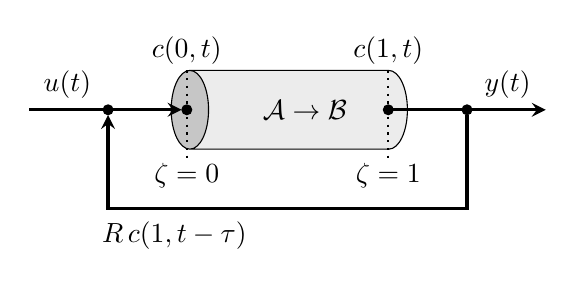
\begin{tikzpicture}
        \node (pfr) [cylinder, draw, minimum height=3cm, minimum width=1cm, shape aspect=1, shape border rotate=180, cylinder uses custom fill, cylinder end fill=gray!45, cylinder body fill=gray!15] {$\mathcal{A} \rightarrow \mathcal{B}$};
        \node (pfr_inlet) [circle, left of=pfr, xshift=-0.5cm, fill=black, draw, inner sep=0pt, minimum size=0.25cm, scale=0.5] {};
        \node (pfr_outlet) [circle, at={(pfr.east)}, shift={(-0.25cm,0)}, fill=black, draw, inner sep=0pt, minimum size=0.25cm, scale=0.5] {};
        \node (recycle_right) [circle, right of=pfr_outlet, fill=black, draw, inner sep=0pt, minimum size=0.25cm, scale=0.5] {};
        \node (recycle_left) [circle, left of=pfr_inlet, fill=black, draw, inner sep=0pt, minimum size=0.25cm, scale=0.5] {};
    
        \draw[dotted, thick] ([yshift=0.5cm]pfr_inlet.center) -- node[at end, below, yshift=0.1cm] {$\zeta = 0$} ([yshift=-0.65cm]pfr_inlet.center);
        \draw[dotted, thick] ([yshift=0.5cm]pfr_outlet.center) -- node[at end, below, yshift=0.1cm] {$\zeta = 1$} ([yshift=-0.65cm]pfr_outlet.center);
    
        \node[below of=recycle_left, node distance=1.3cm, anchor=north west, xshift=-0.2cm] {$R \, c(1, t-\tau)$};
        \node[above of=pfr_inlet, node distance=0.75cm,] {$c(0, t)$};
        \node[above of=pfr_outlet, node distance=0.75cm,] {$c(1, t)$};
        
        \draw [arrow_2] (pfr_outlet) -- node[near end, above] {$y(t)$} ++(2,0);
        \draw [arrow_2] (pfr_inlet) ++(-2,0) coordinate(start) -- node[near start, above] {$u(t)$} (pfr_inlet);
        \draw [arrow_2] (recycle_right) -- ++(0,-1.25) -| (recycle_left);
        
    \end{tikzpicture}
    \caption{Axial tubular reactor with recycle stream.}
    \label{fig:reactor_scheme}
\end{figure}

% \begin{figure}[!htbp]
%     \centering
%     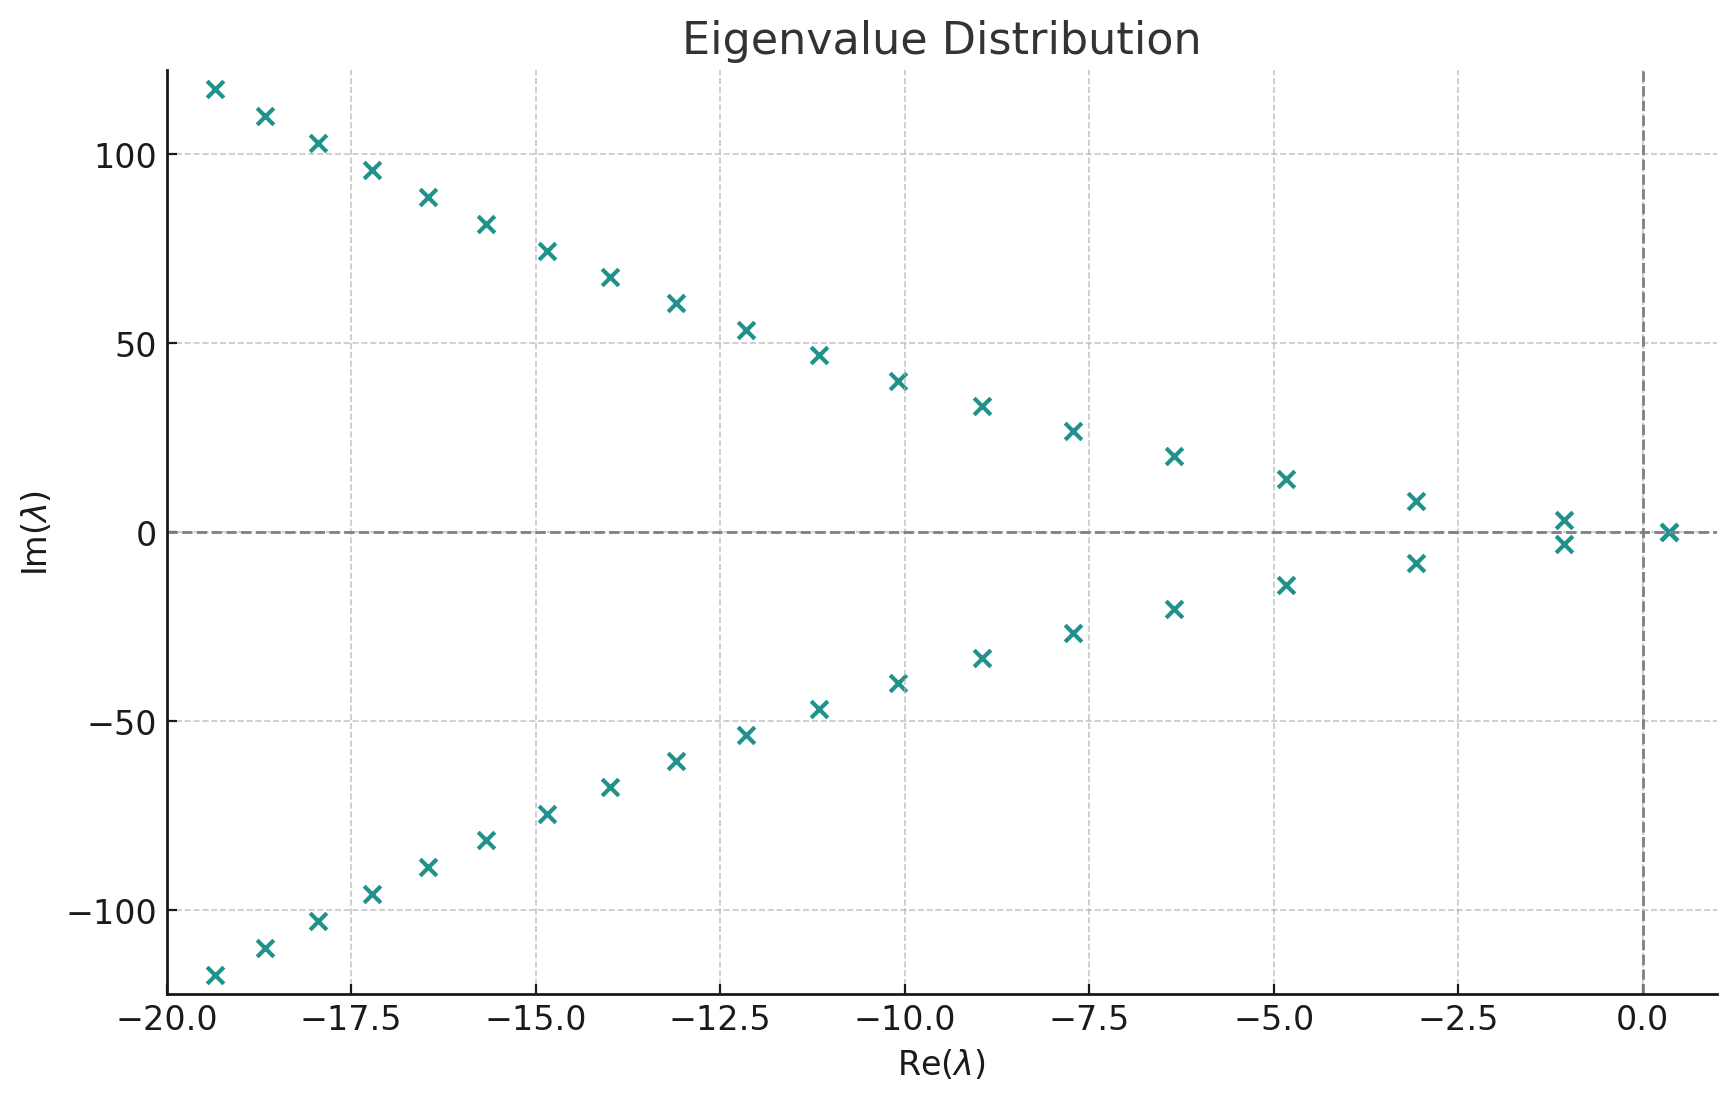
\includegraphics[width=0.7\textwidth]{Figures/eigval_dist_R_0.3.jpg}
%     \caption{Eigenvalues of operator $\mathfrak{A}$ obtained by solving Equation~(\ref{eq:eigval_calc_4}).}
%     \label{fig:eigval_dist}
% \end{figure}

\begin{figure}[!htbp]
    \centering
    \includesvg[inkscapelatex=false, width=0.8\textwidth, keepaspectratio]{Figures/eig_val_dist_R_0.3.svg}
    \caption{Eigenvalues of operator $\mathfrak{A}$ obtained by solving Equation~(\ref{eq:eigval_calc_4}).}
    \label{fig:eigval_dist}
\end{figure}

% \begin{figure}[!htbp]
%     \centering
%     \includesvg[inkscapelatex=false, width=0.8\textwidth, keepaspectratio]{Figures/eigval_dist_R_0.3.svg}
%     \caption{Eigenvalues of operator $\mathfrak{A}$ obtained by solving Equation~(\ref{eq:eigval_calc_4}).}
%     \label{fig:eigval_dist}
% \end{figure}

\begin{figure}[!htbp]
    \centering
    \includesvg[inkscapelatex=false, width=0.6\textwidth, keepaspectratio]{Figures/eigfuns.svg}
    \caption{First few eigenmodes of $\mathfrak{A}$ and $\mathfrak{A}^*$.}
    \label{fig:eigfun}
\end{figure}

\begin{figure}[!htbp]
    \centering
    \begin{subfigure}[b]{0.45\textwidth}
        \centering
        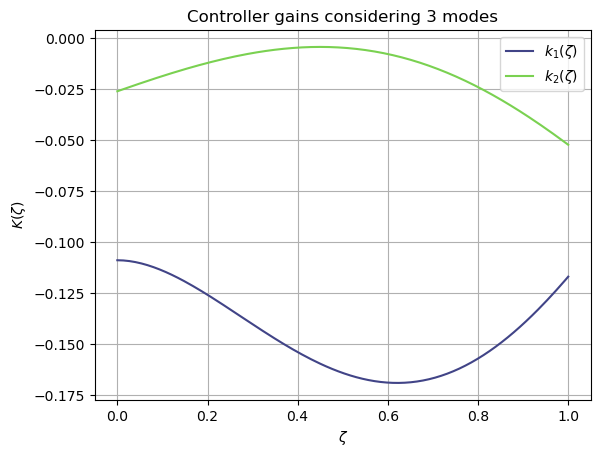
\includegraphics[width=\textwidth]{Figures/k_3.png}
        \caption{$N = 3$}
        \label{fig:k_3}
    \end{subfigure}
    \hfill
    \begin{subfigure}[b]{0.45\textwidth}
        \centering
        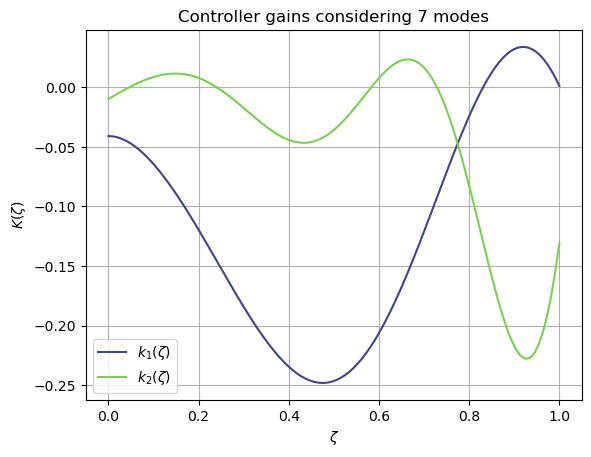
\includegraphics[width=\textwidth]{Figures/k_7.png}
        \caption{$N = 7$}
        \label{fig:k_7}
    \end{subfigure}
    \caption{Full-state feedback gain $\bm{K}(\zeta)$ utilizing the first $N$ modes of the system given by Equation~(\ref{eq:fullstate_gain}).}
    \label{fig:k_modes}
\end{figure}

\begin{figure}[!htbp]
    \centering
    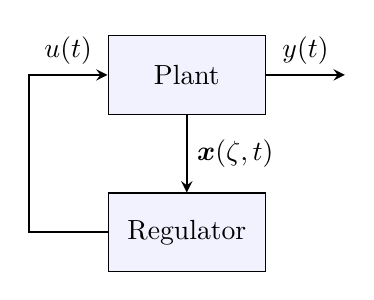
\begin{tikzpicture}[node distance=2cm]
        \node (plant) [block_1] {Plant};
        \node (regulator) [block_1, below of=plant] {Regulator};
        \draw [arrow] (plant.south) -- node[midway, right] {$\bm{x}(\zeta,t)$} (regulator.north);
        \draw [arrow] (regulator.west) -- ++(-1,0) |- node[near end, above] {$u(t)$} (plant.west);
        \draw [arrow] (plant.east) -- node[midway, above] {$y(t)$} ++(1,0);
    \end{tikzpicture}
    \caption{Block diagram representation of the optimal full-state feedback control system.}
    \label{fig:block_diagram}
\end{figure}

\begin{figure}[!htbp]
    \centering
    \includesvg[inkscapelatex=false, width=0.5\textwidth, keepaspectratio]{Figures/L.svg}
    \caption{Observer gain $\bm{L}(\zeta)$.}
    \label{fig:L_modes}
\end{figure}

\begin{figure}[!htbp]
    \centering
    \includesvg[inkscapelatex=false, width=0.5\textwidth, keepaspectratio]{Figures/pole_placement.svg}
    \caption{Eigenvalues of the observer-based controller, full-state feedback controller, and open-loop system.}
    \label{fig:eigs}
\end{figure}

\begin{figure}[!htbp]
    \centering
    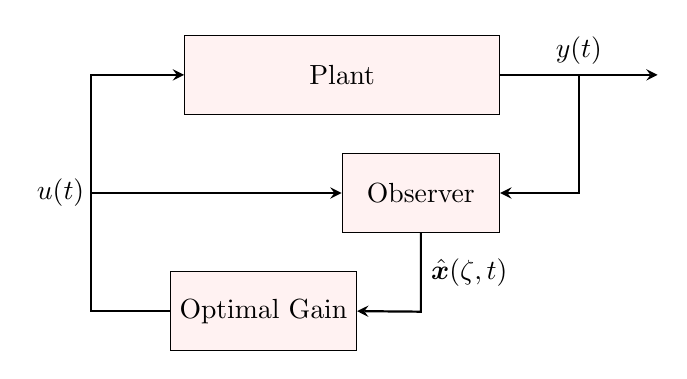
\begin{tikzpicture}[node distance=2cm]
        \node (plant) [block_2, minimum width=4cm] {Plant};
        \node (regulator) [block_2, below of=plant, xshift=-1cm, yshift=-1cm] {Optimal Gain};
        \node (observer) [block_2, below of=plant, xshift=1cm, yshift=0.5cm] {Observer};
        \draw [arrow] (plant.east) -- node[midway, above] {$y(t)$} ++(2,0);
        \draw [arrow] (plant.east) ++(1,0) |- (observer.east);
        \draw [arrow] (observer.south) -- ++(0,-1) node[midway, right] {$\hat{\bm{x}}(\zeta,t)$} -- (regulator.east);    
        \draw [arrow] (regulator.west) -- ++(-1,0) |- (plant.west);
        \draw [arrow] (regulator.west) ++(-1,1.5) coordinate(start) -- node[near start, left, xshift=-0.75cm] {$u(t)$} (observer.west);
    \end{tikzpicture}
    \caption{Block diagram representation of the observer-based output feedback control system.}
    \label{fig:block_diagram_observer}
\end{figure}

\begin{figure}[!htbp]
    \centering
    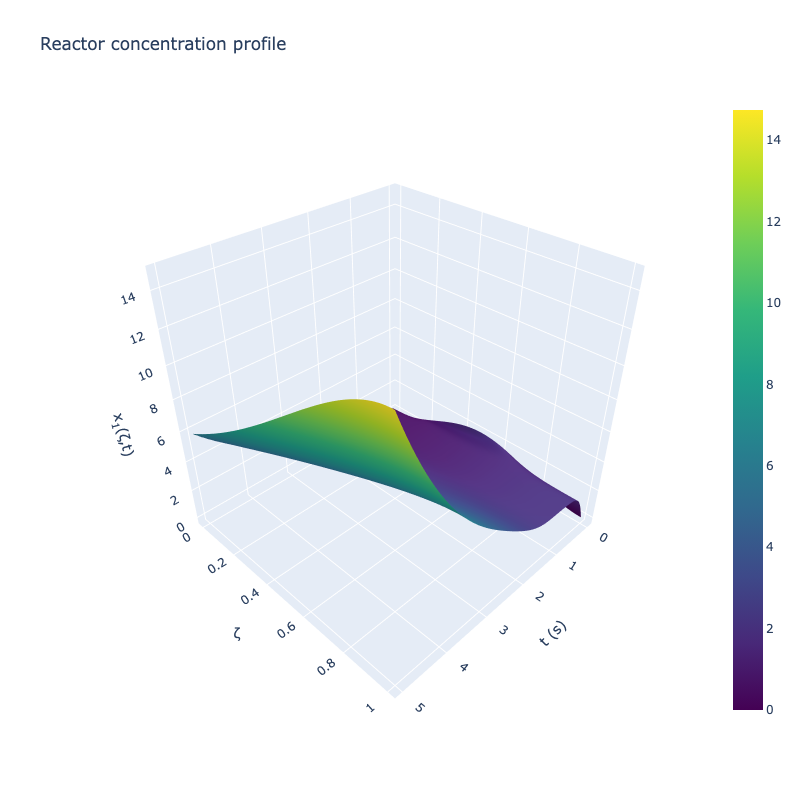
\includegraphics[width=0.8\textwidth,trim=0 0 100 0,clip]{Figures/3D_x1_openloop.png}
    \caption{Zero-input response of the unstable open-loop system as described by Equations~(\ref{eq:PDE_original_model})~and~(\ref{eq:BC}).}
    \label{fig:3D_x1_openloop}
\end{figure}

\begin{figure}[!htbp]
    \centering
    \begin{subfigure}[b]{0.45\textwidth}
        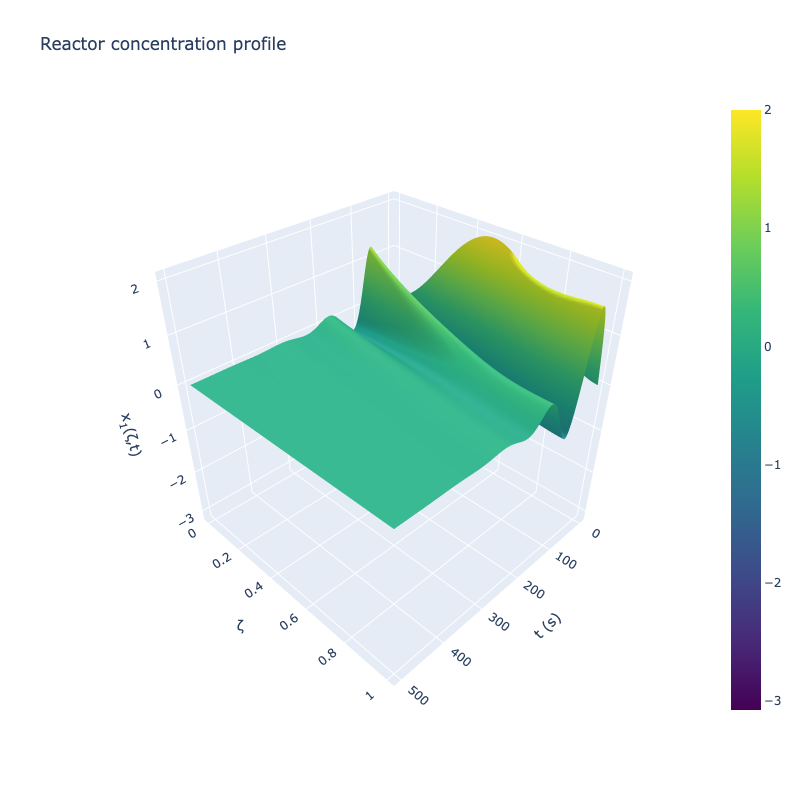
\includegraphics[width=\textwidth,trim=0 0 100 0,clip]{Figures/3D_x1_k3.png}
        \caption{$N=3$}
        \label{fig:3D_x1_k3}
    \end{subfigure}
    \hfill
    \begin{subfigure}[b]{0.45\textwidth}
        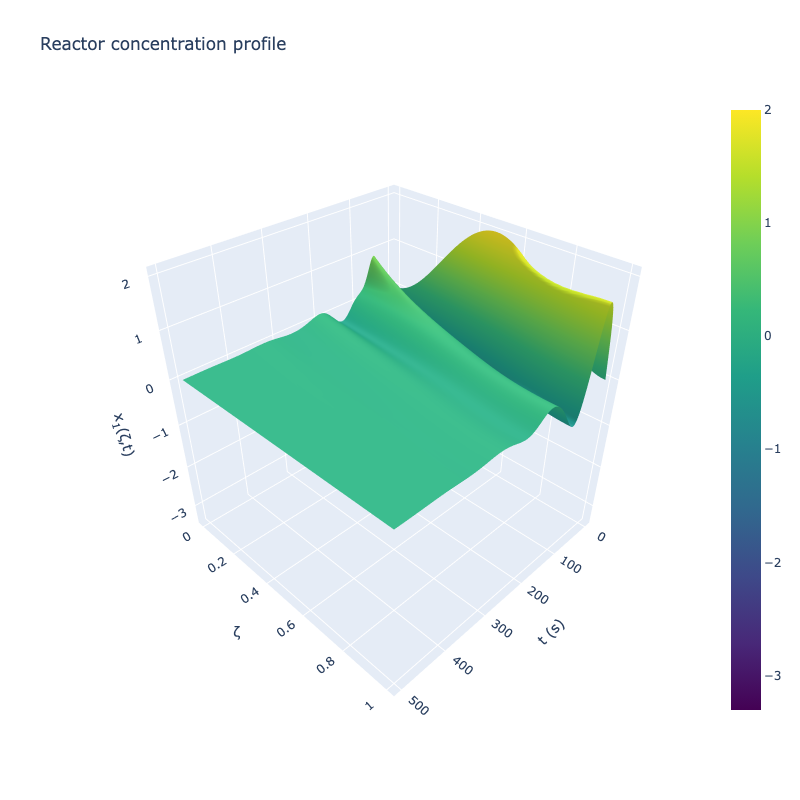
\includegraphics[width=\textwidth,trim=0 0 100 0,clip]{Figures/3D_x1_k7.png}
        \caption{$N=7$}
        \label{fig:3D_x1_k7}
    \end{subfigure}
    \caption{Input response of the system under full-state feedback control given by Equation~(\ref{eq:fullstate_ss}), utilizing the feedback gain obtained in Figure~\ref{fig:k_modes}.}
    \label{fig:full_state_feedback}
\end{figure}

\begin{figure}[!htbp]
    \centering
    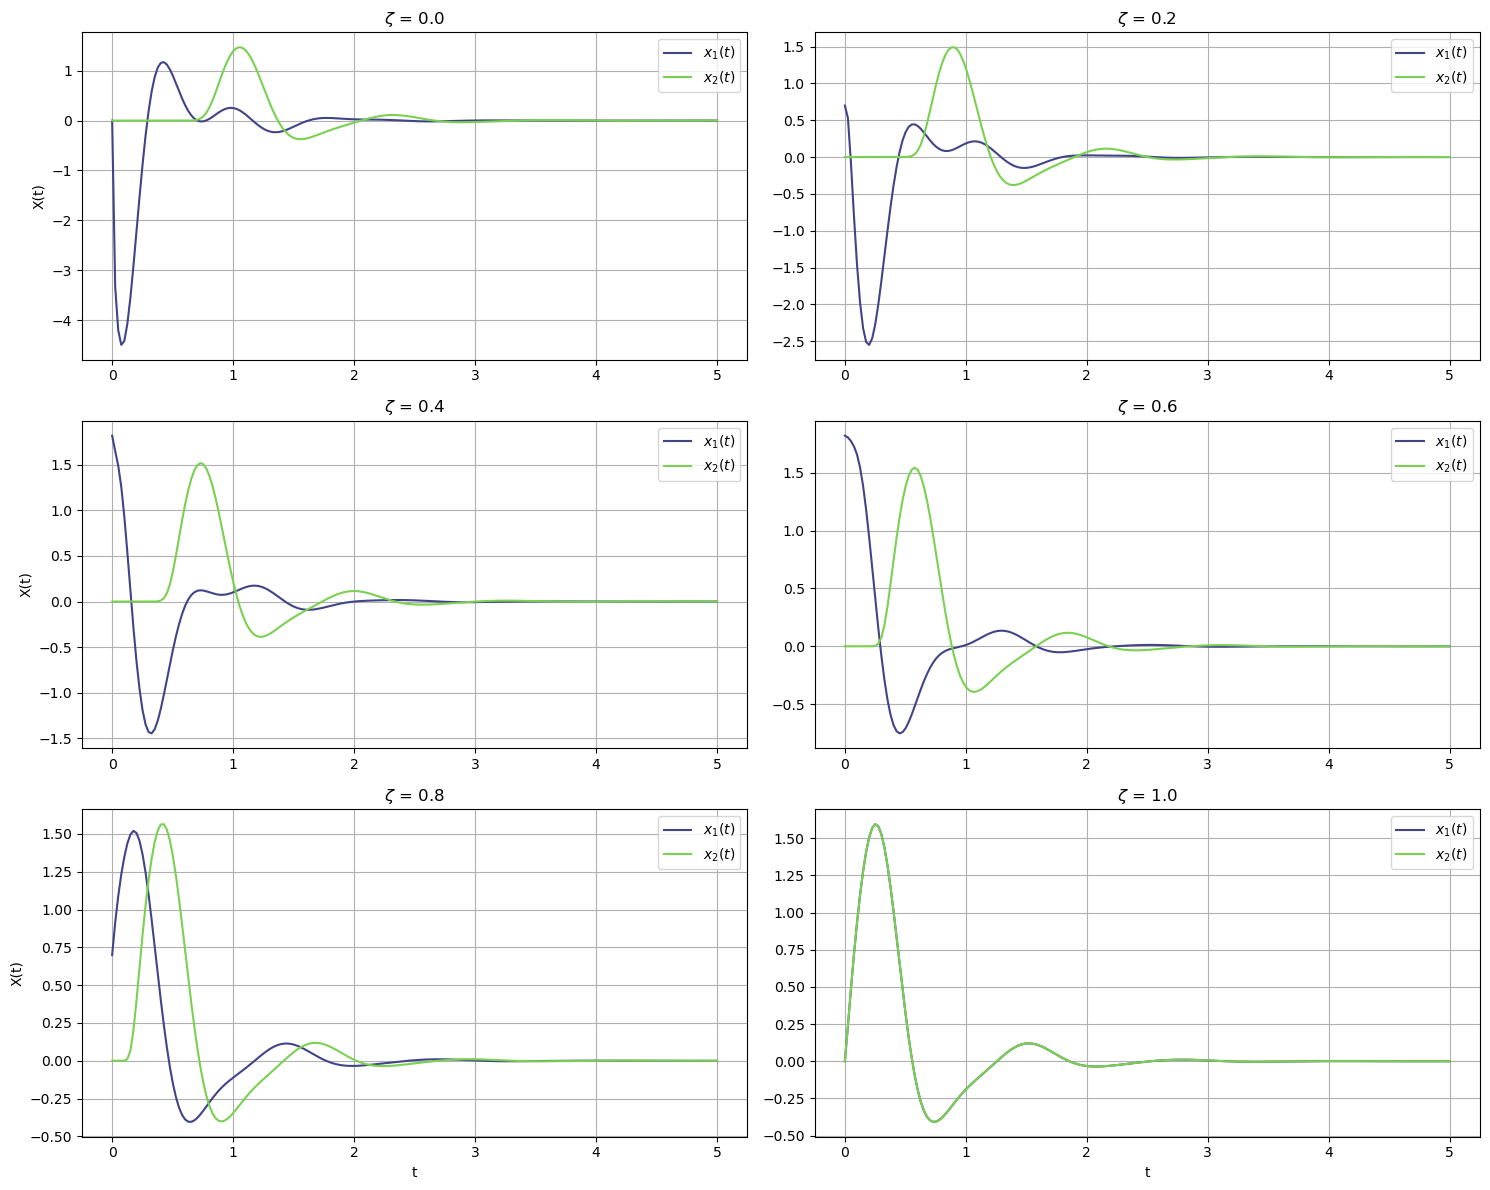
\includegraphics[width=0.8\textwidth]{Figures/2D_xt_k7.png}
    \caption{2D cross-section plots of the full-state feedback input response at various $\zeta$ positions, utilizing the feedback gain obtained in Figure~\ref{fig:k_7}.}
    \label{fig:2D_xt_k7}
\end{figure}

\begin{figure}[!htbp]
    \centering
    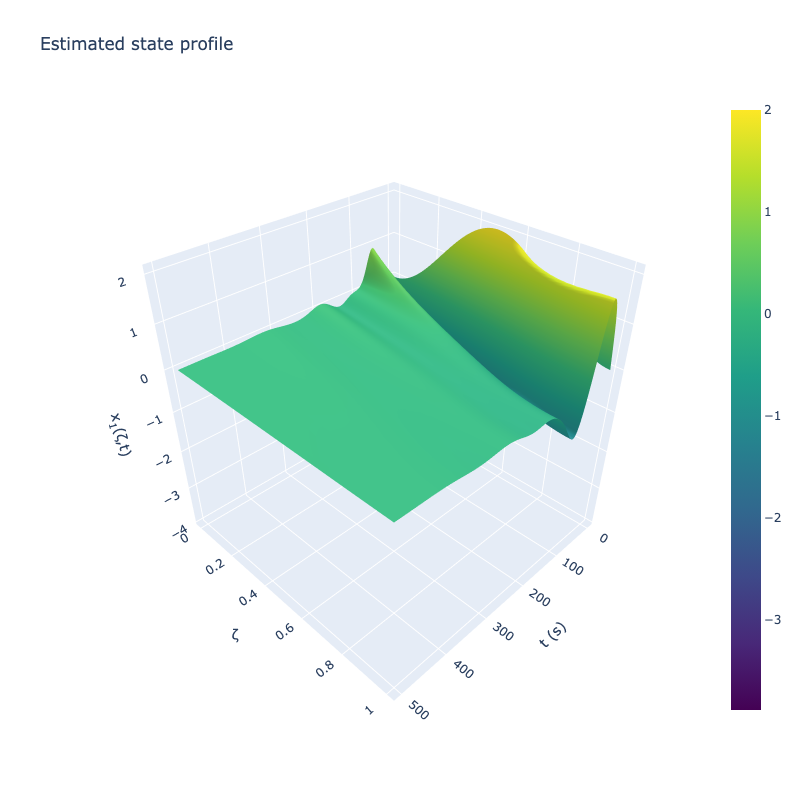
\includegraphics[width=0.8\textwidth,trim=0 0 100 0,clip]{Figures/3D_x1_L_k7.png}
    \caption{Input response of the system under observer-based output feedback control given by Equation~(\ref{eq:observer_ss}), utilizing the observer gain obtained in Figure~\ref{fig:L_modes} and the feedback gain obtained in Figure~\ref{fig:k_7}.}
    \label{fig:3D_x1_L_k7}
\end{figure}

\begin{figure}[!htbp]
    \centering
    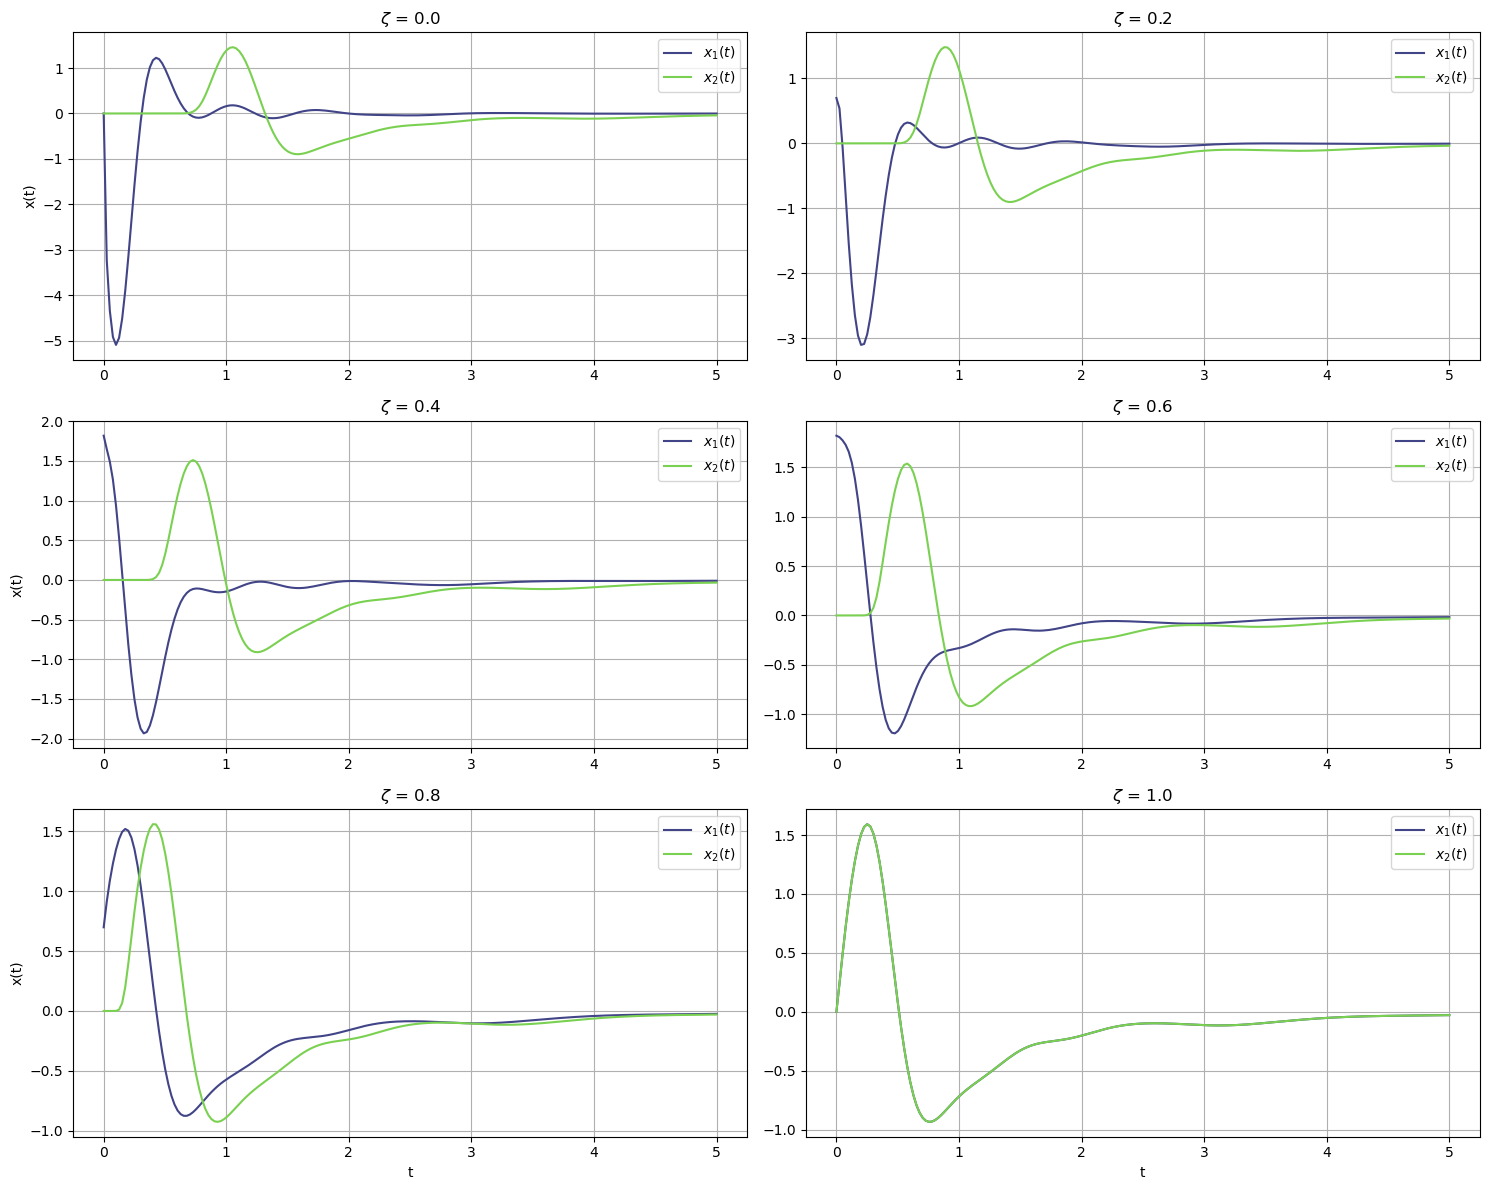
\includegraphics[width=0.8\textwidth]{Figures/2D_xt_L_k7.png}
    \caption{2D cross-section plots of the input response at various $\zeta$ positions, utilizing the observer gain obtained in Figure~\ref{fig:L_modes} and the feedback gain obtained in Figure~\ref{fig:k_7}.}
    \label{fig:2D_xt_L_k7}
\end{figure}

\begin{figure}[!htbp]
    \centering
    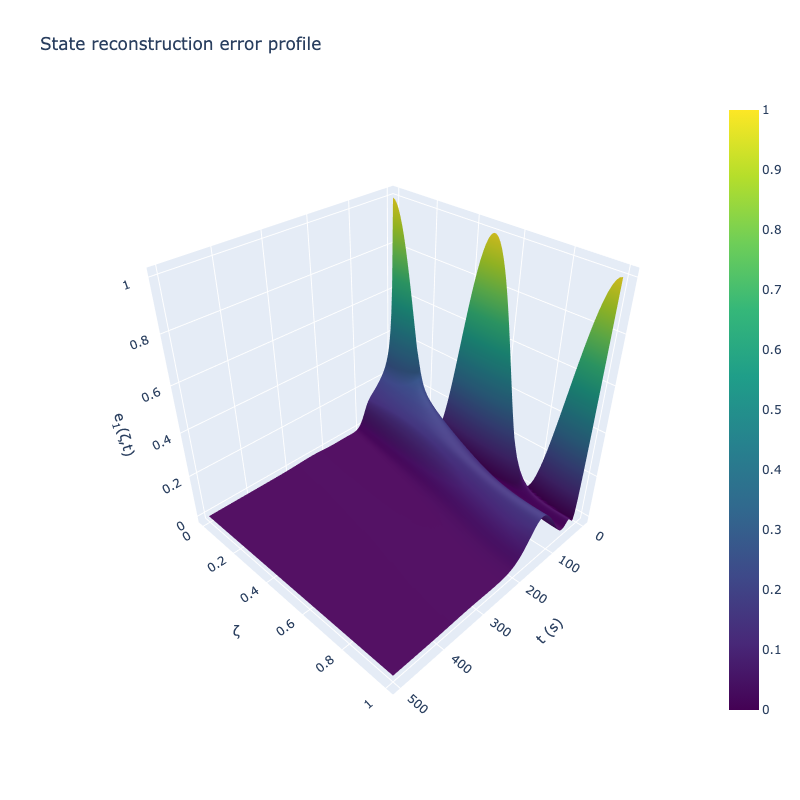
\includegraphics[width=0.8\textwidth,trim=0 0 100 0,clip]{Figures/3D_e1_L_k7.png}
    \caption{Error dynamics of the observer-based regulator utilizing the observer gain obtained in Figure~\ref{fig:L_modes} and the feedback gain obtained in Figure~\ref{fig:k_7}.}
    \label{fig:3D_e1_L_k7}
\end{figure}

\begin{figure}[!htbp]
    \centering
    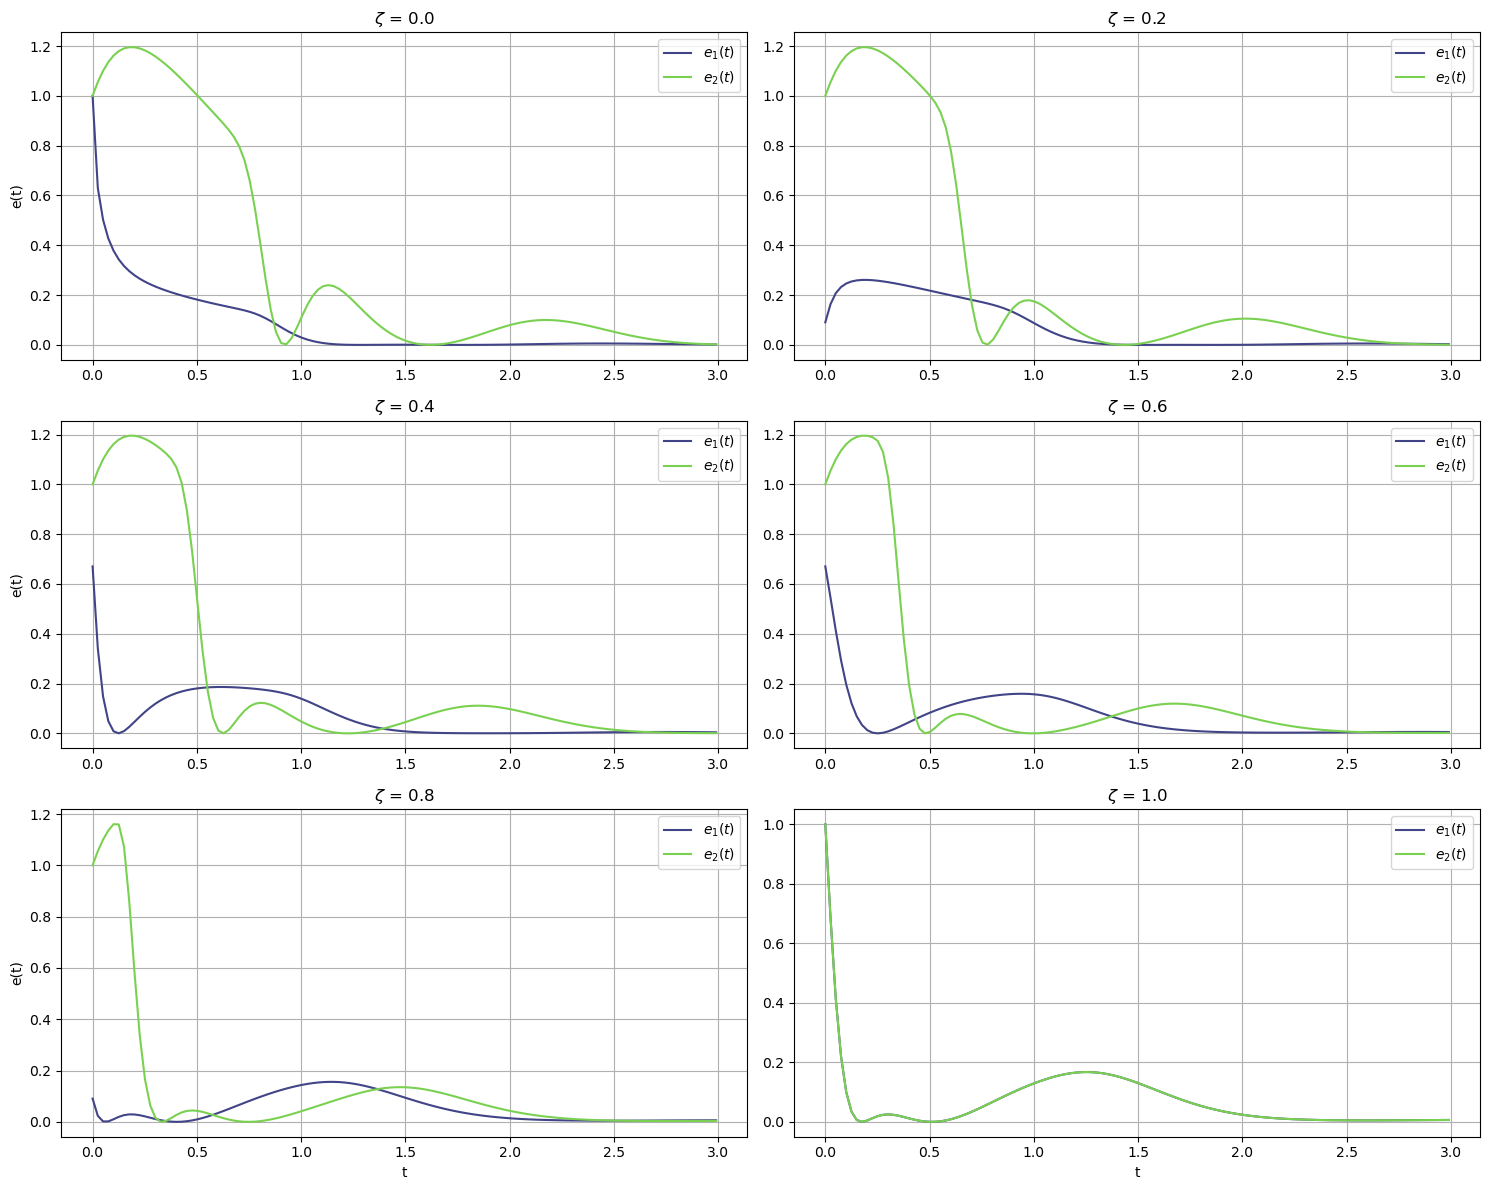
\includegraphics[width=0.8\textwidth]{Figures/2D_et_L_k7.png}
    \caption{2D cross-section plots of the error dynamics of the observer-based regulator at various $\zeta$ positions, utilizing the observer gain obtained in Figure~\ref{fig:L_modes} and the feedback gain obtained in Figure~\ref{fig:k_7}.}
    \label{fig:2D_et_L_k7}
\end{figure}


\end{document}
